%%%%%%%%%%%%%%%%%%%%%%%%%%%%%%%%%%%%%%%%%%%%%%%%%%%%%%%%%%%%%%%%%%%%%%%%%%%%
% AGUJournalTemplate.tex: this template file is for articles formatted with LaTeX
%
% This file includes commands and instructions
% given in the order necessary to produce a final output that will
% satisfy AGU requirements, including customized APA reference formatting.
%
% You may copy this file and give it your
% article name, and enter your text.
%
% guidelines and troubleshooting are here: 

%% To submit your paper:
\documentclass[draft]{agujournal2019}
\usepackage{url} %this package should fix any errors with URLs in refs.
\usepackage{lineno}
\usepackage[inline]{trackchanges} %for better track changes. finalnew option will compile document with changes incorporated.
\usepackage{soul}
\usepackage{multirow} % add this in your preamble
\usepackage{bigdelim} % for curly braces in tables

\linenumbers
%%%%%%%
% As of 2018 we recommend use of the TrackChanges package to mark revisions.
% The trackchanges package adds five new LaTeX commands:
%
%  \note[editor]{The note}
%  \annote[editor]{Text to annotate}{The note}
%  \add[editor]{Text to add}
%  \remove[editor]{Text to remove}
%  \change[editor]{Text to remove}{Text to add}
%
% complete documentation is here: http://trackchanges.sourceforge.net/
%%%%%%%

% \draftfalse

%% Enter journal name below.
%% Choose from this list of Journals:
%
% JGR: Atmospheres
% JGR: Biogeosciences
% JGR: Earth Surface
% JGR: Oceans
% JGR: Planets
% JGR: Solid Earth
% JGR: Space Physics
% Global Biogeochemical Cycles
% Geophysical Research Letters
% Paleoceanography and Paleoclimatology
% Radio Science
% Reviews of Geophysics
% Tectonics
% Space Weather
% Water Resources Research
% Geochemistry, Geophysics, Geosystems
% Journal of Advances in Modeling Earth Systems (JAMES)
% Earth's Future
% Earth and Space Science
% Geohealth
%
% ie, \journalname{Water Resources Research}

\journalname{JGR: Oceans}


\begin{document}

%%%%%%%%%%%%%%%%%%%%%%%%%%%%%%%%%%%%%%%%%%%%%%%
%  TITLE
%
% (A title should be specific, informative, and brief. Use
% abbreviations only if they are defined in the abstract. Titles that
% start with general keywords then specific terms are optimized in
% searches)
%
%%%%%%%%%%%%%%%%%%%%%%%%%%%%%%%%%%%%%%%%%%%%%%%

% Example: \title{This is a test title}

\title{Evidence of Synoptic Cross-shelf Pathways of Mid-depth Salinity Maximum Intrusions in the South Brazil Bight}

%%%%%%%%%%%%%%%%%%%%%%%%%%%%%%%%%%%%%%%%%%%%%%%
%
%  AUTHORS AND AFFILIATIONS
%
%%%%%%%%%%%%%%%%%%%%%%%%%%%%%%%%%%%%%%%%%%%%%%%

% Authors are individuals who have significantly contributed to the
% research and preparation of the article. Group authors are allowed, if
% each author in the group is separately identified in an appendix.)

% List authors by first name or initial followed by last name and
% separated by commas. Use \affil{} to number affiliations, and
% \thanks{} for author notes.
% Additional author notes should be indicated with \thanks{} (for
% example, for current addresses).

% Example: \authors{A. B. Author\affil{1}\thanks{Current address, Antartica}, B. C. Author\affil{2,3}, and D. E.
% Author\affil{3,4}\thanks{Also funded by Monsanto.}}

\authors{D. A. Silva\affil{1}, A. Gangopadhyay\affil{2}, D. K. Sasaki\affil{1,3}, M. Dottori\affil{1}, I. C. A. da Silveira\affil{1}, W. C. Belo\affil{4}, R. P. Martins\affil{4}}

\affiliation{1}{Instituto Oceanogr\'{a}fico, Universidade de Sao Paulo, Praca do Oceanogr\'{a}fico, 191 - SP 05508-120, S\~{a}o Paulo, Brasil}

\affiliation{2}{School for Marine Sciences and Technology, University of Massachusetts, 836 South Rodney French Blvd, New Bedford, MA 02744-1221}

\affiliation{3}{Department of Marine and Environmental Sciences, Northeastern University, 430 Nahant Rd, Nahant, MA 01908}

\affiliation{4}{Centro de Pesquisas, Desenvolvimento e Inova\c{c}\~{a}o Leopoldo Am\'{e}rico Miguez de Mello - CENPES/PETROBRAS, Av. Hor\'{a}cio Macedo, 950 - Cidade Universit\'{a}ria da Universidade Federal do Rio de Janeiro, Rio de Janeiro - RJ, 21941-915}

%(repeat as many times as is necessary)


% Corresponding author mailing address and e-mail address:

% (include name and email addresses of the corresponding author.  More
% than one corresponding author is allowed in this LaTeX file and for
% publication; but only one corresponding author is allowed in our
% editorial system.)

% Example: \correspondingauthor{First and Last Name}{email@address.edu}

\correspondingauthor{Danilo Silva}{danilo2.silva@usp.br}



%%%%%%%%%%%%%%%%%%%%%%%%%%%%%%%%%%%%%%%%%%%%%%%
% KEY POINTS
%%%%%%%%%%%%%%%%%%%%%%%%%%%%%%%%%%%%%%%%%%%%%%%
%  List up to three key points (at least one is required)
%  Key Points summarize the main points and conclusions of the article
%  Each must be 140 characters or fewer with no special characters or punctuation and must be complete sentences

% Example:
% \begin{keypoints}
% \item	List up to three key points (at least one is required)
% \item	Key Points summarize the main points and conclusions of the article
% \item	Each must be 140 characters or fewer with no special characters or punctuation and must be complete sentences
% \end{keypoints}

\begin{keypoints}
\item We present evidence that the observed Salinity Maximum intrusions (\textit{$S_{max}$}) in the South Brazil Bight (SBB) are remotely advected from north and east of SBB, where the intrusions originate.
\item We found the Cabo Frio Eddy (CFE) was the main mechanism for advecting the \textit{$S_{max}$} towards the shelf break, while Ekman transport pushed these intrusions into the shelf.
\item Two other secondary processes, enhancement by Agulhas Rings and advection through a non-meandering Brazil Current are also identified.
\end{keypoints}

%%%%%%%%%%%%%%%%%%%%%%%%%%%%%%%%%%%%%%%%%%%%%%%
%
%  ABSTRACT and PLAIN LANGUAGE SUMMARY
%
% A good Abstract will begin with a short description of the problem
% being addressed, briefly describe the new data or analyses, then
% briefly states the main conclusion(s) and how they are supported and
% uncertainties.

% The Plain Language Summary should be written for a broad audience,
% including journalists and the science-interested public, that will not have 
% a background in your field.
%
% A Plain Language Summary is required in GRL, JGR: Planets, JGR: Biogeosciences,
% JGR: Oceans, G-Cubed, Reviews of Geophysics, and JAMES.
% see http://sharingscience.agu.org/creating-plain-language-summary/)
%
%%%%%%%%%%%%%%%%%%%%%%%%%%%%%%%%%%%%%%%%%%%%%%%

%% \begin{abstract} starts the second page

\begin{abstract}
Cross-shelf exchanges play a crucial role in distributing heat, salt, pollutants, and biogeochemical properties between the continental shelf and the open ocean. Among the processes shaping these exchanges, the intrusion of salty and warm waters (mid-depth Salinity Maximum, \textit{$S_{max}$}) remains poorly understood in the South Brazil Bight (SBB). Here, we present observational evidence of \textit{$S_{max}$} intrusions in the Northeast SBB (NE-SBB) from independent measurements between February and March 2022. The dataset identified the Cabo Frio Eddy (CFE) as the main mechanism driving a cross-shelf pathway to the shelf break, with advection further enhanced by interaction with an Agulhas Ring (AgR). Backward Lagrangian analysis confirmed this pathway and traced the origin of \textit{$S_{max}$} to northeastern locations outside the NE-SBB. It also suggested an additional southwestward along-shelf pathway, resembling the non-meandering Brazil Current, directly advecting \textit{$S_{max}$} from their source region. In both cases, once \textit{$S_{max}$} reached the shelf break, Burger number (Bu) analysis revealed an onshore counterflow at mid-depths (Bu $>$ 1), driven by wind-induced circulation and reinforced by mesoscale dynamics. These findings highlight the role of the CFE in connecting offshore waters to the shelf and emphasize the importance of remote intrusions in shaping the thermodynamics and biogeochemistry of the SBB.
\end{abstract}

\section*{Plain Language Summary}
This study examines the movement of warm, salty water (Salinity Maximum intrusions, \textit{$S_{max}$}) between the continental shelf and the open ocean in the South Brazil Bight (SBB). In early 2022, researchers observed these water intrusions in the northeastern SBB, noting that they primarily travel across the shelf from the southeast, influenced by the Brazil Current. Additionally, some of this water also moves along the shelf. Wind-driven currents create an onshore flow at subsurface levels, which is strengthened by the Brazil Current's dynamics. These findings provide new insights into water movement in the SBB and its impact on marine processes, highlighting the need for further research to better understand these mechanisms.

%%%%%%%%%%%%%%%%%%%%%%%%%%%%%%%%%%%%%%%%%%%%%%%
%
%  BODY TEXT
%
%%%%%%%%%%%%%%%%%%%%%%%%%%%%%%%%%%%%%%%%%%%%%%%

\section{Introduction}
\label{sec:introduction}

Cross-shelf exchanges are critical processes that influence the distribution of heat, salt, pollutants \cite{brink2016} and biogeochemical properties \cite{liu2010carbon,cossarini2015continental} between the continental shelf and the open ocean. Western boundary currents (WBCs), such as the Brazil Current (BC), play an important role in these exchanges because of their dynamic nature and the transport of warm, saline waters poleward along the western margins of ocean basins. 

The Northeastern South Brazil Bight (NE-SBB, Figure~\ref{fig:study_area}) exhibits a secondary maximum of eddy kinetic energy (eKE) in the South Atlantic Basin \cite<refer to Figure 1 from >{rocha2022}. This elevated eKE is related to the quasi-permanent presence of cyclonic eddies generated off Cabo Frio (Cabo Frio Eddy, CFE) and Cabo de São Tomé (Cabo de São Tomé Eddy, CTE) \cite{uchoa2023,silveira2023}. The generation of these eddies results from the topographic interactions of the poleward BC and the equatorward Intermediate Western Boundary Current \cite{luko2022}. The development of meanders and cyclonic eddies influences cross-shelf exchanges \cite{calil2021,combes2023circulation}, in addition to wind-driven cross-shelf circulation \cite{castro2014summer,brink2016}. The on-shelf outcome of these processes over the shelf edge leads to the development of thermohaline intrusions, that is, inversions of temperature and salinity \cite{ruddick-kerr2003}. Although such structures may appear gravitationally unstable, the opposing effects of temperature and salinity on seawater density frequently compensate, allowing intrusions to remain neutrally buoyant \cite{Stern1967}.

\begin{figure}[ht!]
    \centering
    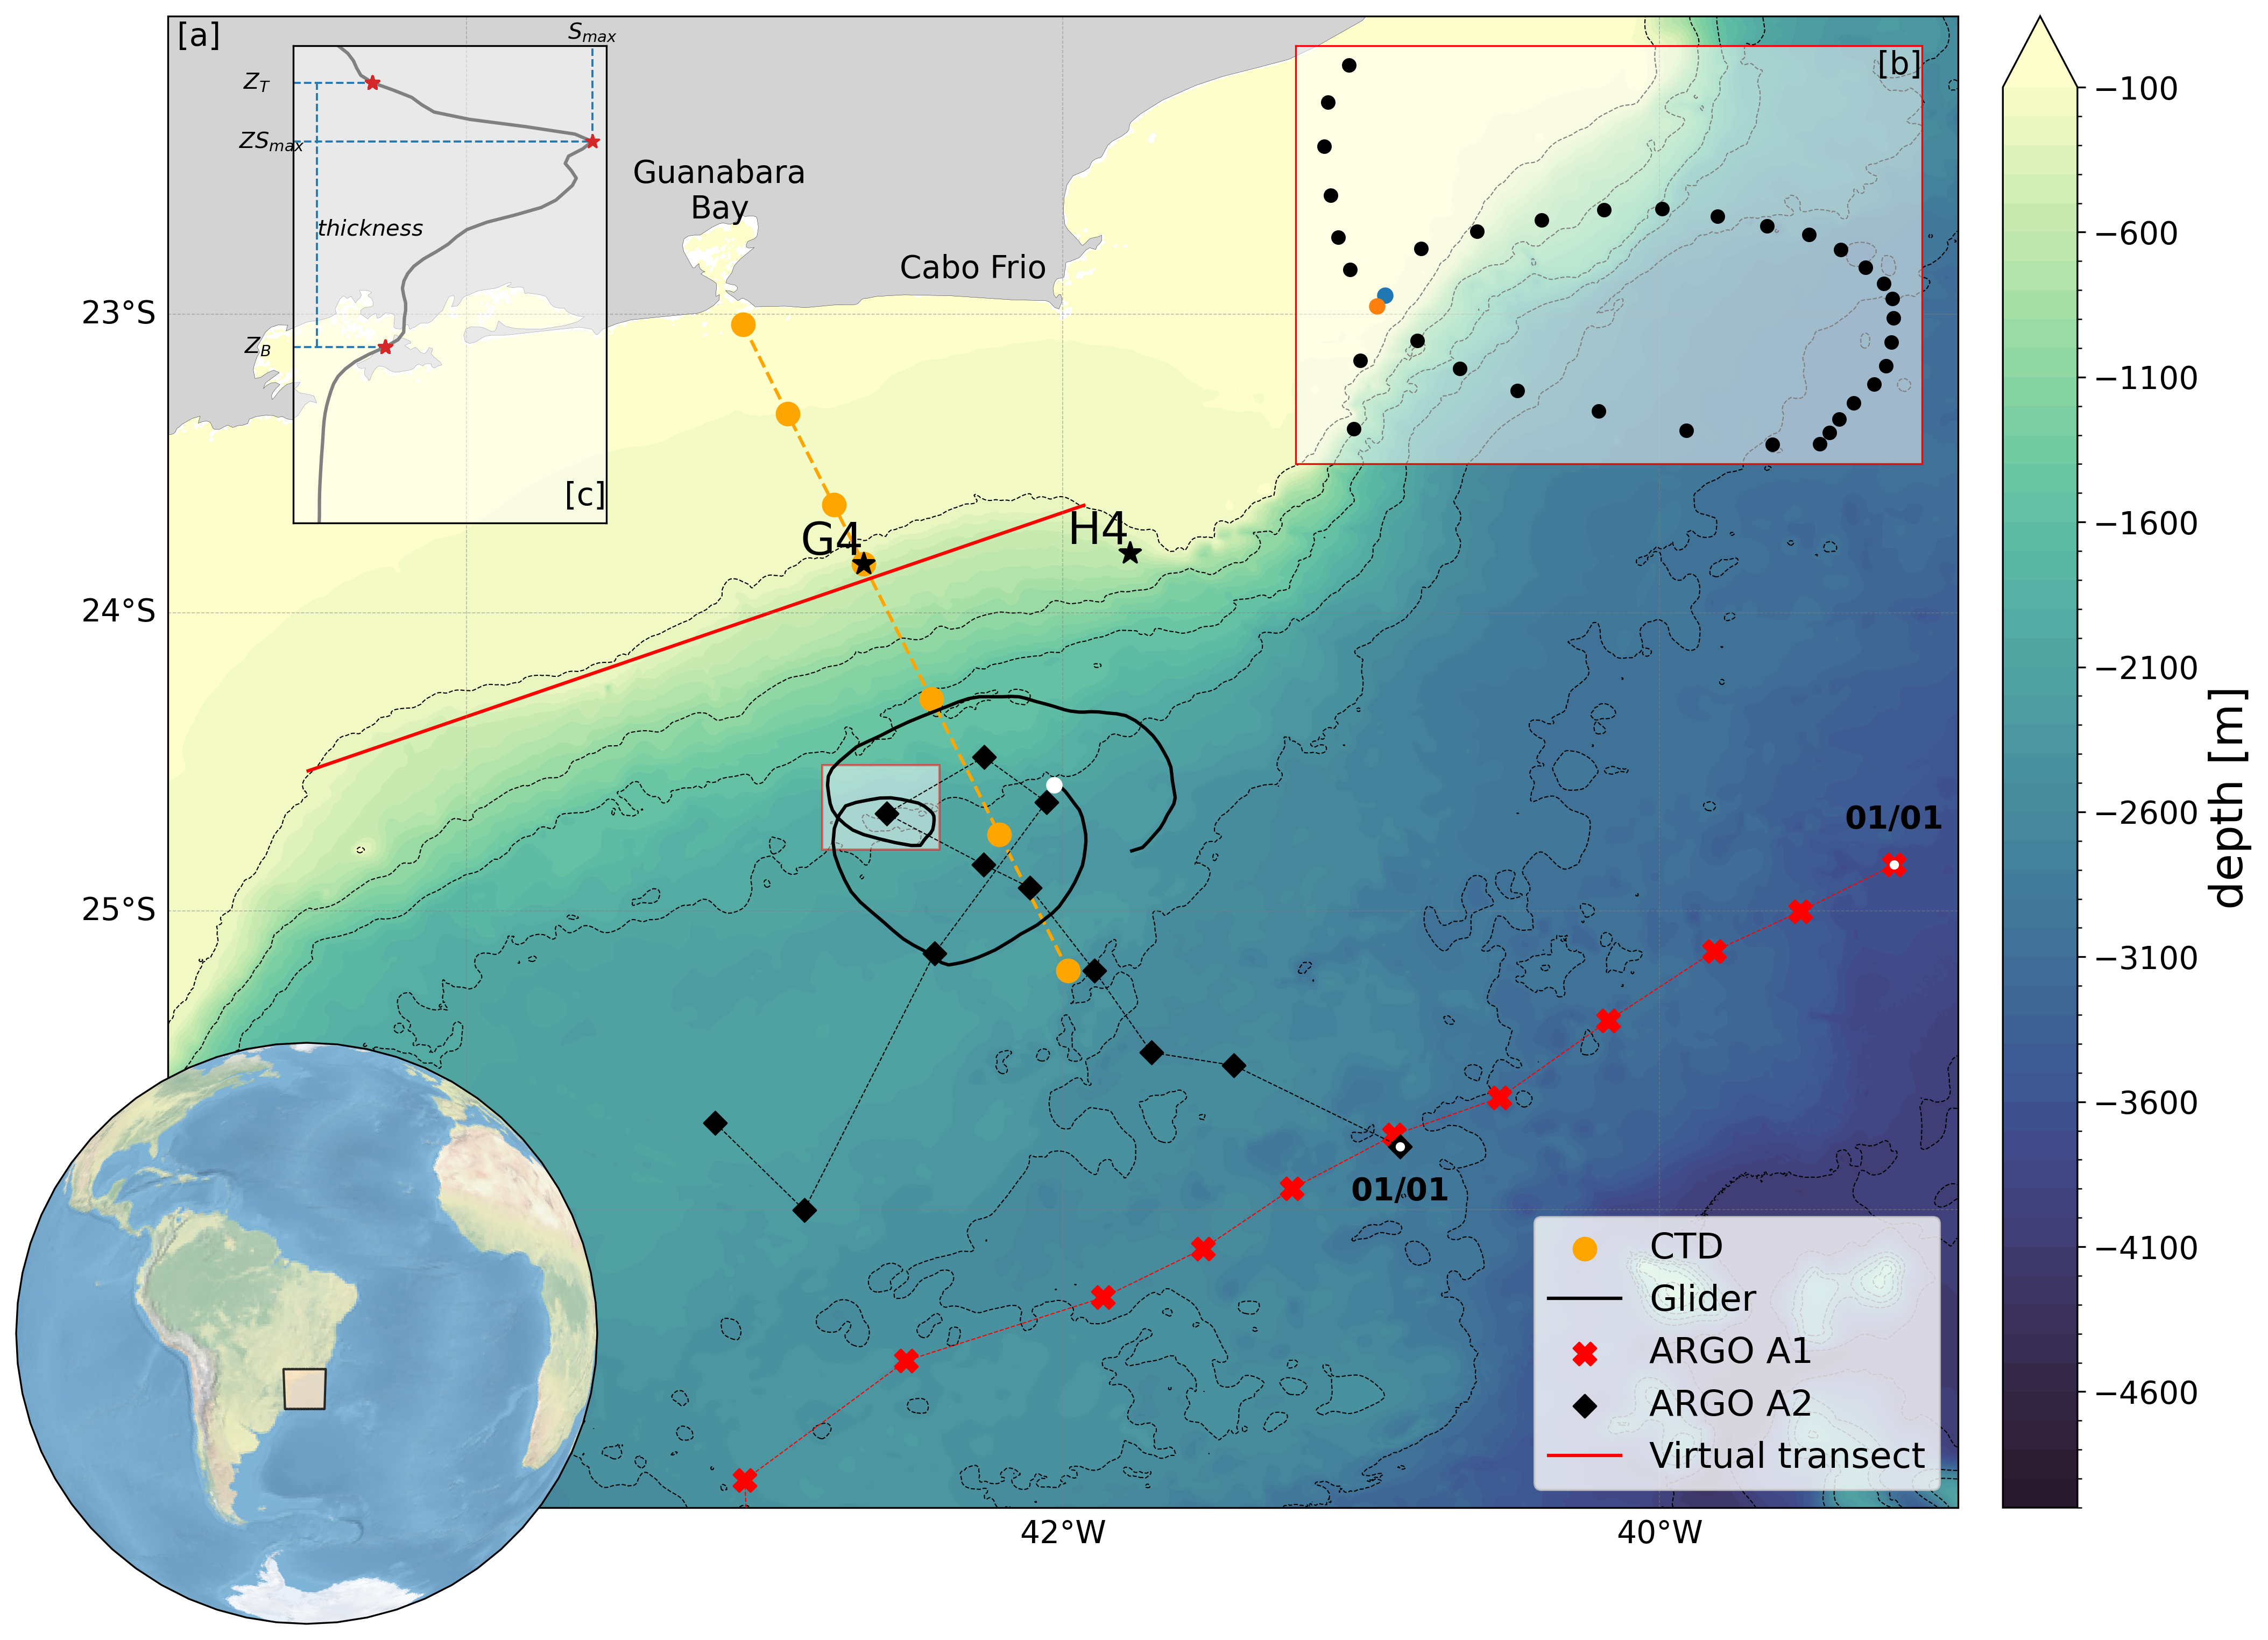
\includegraphics[width=1\linewidth]{figures/00_manuscript_study_area.png}
    \caption{(a) Northeastern South Brazil Bight (NE-SBB) with observational locations in orange representing CTD profiles obtained during the SANAGU2022 cruise; red and black represent ARGO profiles along Line A1 (3901549) and Line A2 (3901225), respectively; the continuous black line represents the Slocum Glider SG19 track depicting the Cabo Frio Eddy (CFE); and the red line represents the along-shelf-edge transect used for cross-shelf velocity calculations. The bathymetric data, marked in color, were extracted from the GEBCO 2019 dataset \protect \cite{weatherall2015new}, and the contours represent the -100, -200, -1000, -2000 and -4000 m isobaths. (b) highlights a specific part of the glider's path in which a loop was performed. The orange and blue dots are two specific profiles measured during the glider's path. (c) Sample absolute salinity profile showing the salinity maximum (\textit{$S_{max}$}) characteristics: $ZS_{max}$ is the depth of the \textit{$S_{max}$}; $Z_{T}$ and $Z_{B}$ are the depths of the top and bottom boundaries, respectively; and $thickness$ is the difference between them. The \textit{$S_{max}$} characteristics were extracted based on the adaptations of the \protect\citeA{Lentz2003} algorithm of \protect\citeA{silva2023inventory}.}
    \label{fig:study_area}
\end{figure}

Thermohaline intrusions can be observed near the bottom, which influence the region by injecting cold and nutrient rich waters (South Atlantic Central Water, SACW) onto the shelf, thus increasing primary productivity and atmospheric CO$_2$ sequestration \cite{oliveira2019first}. However, recent studies have shown a separate intrusion occurring at mid-depth levels that injects warm and salty water onto the shelf \cite<Tropical Water, TW,>{Campos2000,castro2014summer,silva2023inventory}. These intrusions, defined as a peak in subsurface salinity and often called salinity maximum intrusions \cite<hereinafter referred to as $S_{max}$, >{Gordon1981}, sometimes even block the pathway between the nutrient rich waters near the bottom and the euphotic zone \cite{silva2023inventory,dottori2023}, thus affecting the biogeochemical properties of the shelf and the transport of larvae from the ocean \cite{Namiki2017}. These mid-depth salinity maximums, \textit{$S_{max}$}, are generally observed to be associated with seasonal pycnocline \cite{Lentz2003,silva2023inventory} and are responsible for the injection of salt into the shelf. For example, on the Middle Atlantic Bight (MAB), \textit{$S_{max}$} drives the onshore salt flux, providing half of what is necessary to balance the freshwater input and maintain the annual average salinity in the region \cite{Gordon1981}. 

Although thermohaline intrusions are linked to several mechanisms, such as wind- and eddy-driven circulation \cite{Gawarkiewicz1990,GonzalezPola2007,Ruiz2019,Li2012,Malan2020,silver2023increased}, internal waves \cite{Hopkins2012} and baroclinic pressure gradients \cite{Posmentier1978FineFront,Aikman1984}, the drivers of \textit{$S_{max}$} intrusions are still unresolved in the South Brazil Bight (SBB). Considering the dominance of eddies and wind in shaping cross-shelf exchanges \cite{combes2021circulation,calil2021,combes2023circulation}, one might expect that both processes play an important role in developing them. In this study, we investigate the interaction between the dynamics of BC and its eddying meanders and wind-driven circulation and how they might help advect \textit{$S_{max}$} from remote offshore regions all the way to the NE-SBB (Figure~\ref{fig:study_area}). This investigation is motivated by the observation of multiple \textit{$S_{max}$} events advected towards the NE-SBB in March 2022, when the last cruises of the Santos Project - Santos Basin Environmental Characterization - coordinated by PETROBRAS \cite{moreira2023multidisciplinary} were conducted. These cruises were named SANAGU2022.

This study is structured as follows. Section 2 describes the dataset used and methods applied. Section 3 presents our results and shows preferential \textit{$S_{max}$} pathways of advection. Section 4 discusses the interaction between BC dynamics and wind and presents a set of Lagrangian simulations to aid in interpreting the advective pathways. Finally, Section 5 highlights the major conclusions of this study.

\section{Material and Methods}
\label{section:methods}

\subsection{Hydrographic Dataset}
In this study, we use a diverse set of data from several sources, including in situ measurements, remotely sensed products and global numerical reanalysis (as summarized in Table~\ref{tab:dataset}). 

The SANAGU2022 cruises were carried out in March 2022, sampling the entire South Brazil Bight, as described in \citeA{moreira2023multidisciplinary}. Although multiple transects were made on the NE-SBB during the cruise, in this work we only considered the central transect, off Guanabara Bay (Figure~\ref{fig:study_area} orange markers), as intrusions were only observed along this transect. The transect was sampled twice in 2 weeks: the first sample occurred between 5 and 14 March, and the second was performed between 23 and 28 March. CTD profiles measurements were taken with SBE 911 Plus probe, with stations aligned approximately perpendicular to the coast (orange dashed line in Figure~\ref{fig:study_area}). Quality control and processing methods were applied using a modified version of the Python-CTD package \cite{Fernandes2014,dottori2023}. In the processing workflow, we removed spikes, averaged the data into 1 $m$ bin, and applied a 7-point (21-point) window Hanning filter to smooth the profiles over the shelf (slope). This processing is similar to the one applied by \citeA{silva2023inventory} and \citeA{dottori2023} on the same continental shelf and by \citeA{silveira2023} for the slope casts.

\begin{table}
\caption{Overview of the observational datasets used in this study, specifying the source (institution, product name, or reference), extracted variables, and analysis periods. ADT denotes Absolute Dynamic Topography.}
\label{tab:dataset}
\centering
\begin{tabular}{l c c c}
\hline
 \textbf{dataset} & \textbf{source} & \textbf{variables} & \textbf{period} \\
\hline
        CTD           & - & T,S & Mar, 2023 \\ 
        ARGO          & ARGO & T,S & Jan-Mar, 2023 \\ 
        Glider        & ProjetoAzul & T,S & Feb-Mar, 2023 \\ 
        AVISO         & CMEMS & Gridded ADT & \rdelim\}{7}{*}[Jan--Mar, 2023] \\ 
        AVISO         & CMEMS & Along track ADT &  \\ 
        ERA5          & \cite{hersbach2018era5} & Wind stress &  \\ 
        GLORYS12V1    & CMEMS & u,v,T,S &  \\ 
        MERGE         & \cite{rozante2010combining} & Precipitation &  \\ 
        AVHRR         & - & SST &  \\ 
        META3.1exp DT & \cite{pegliasco2022} & Eddie track(x,y,t) &  \\ 
\hline
\end{tabular}
\end{table}

ARGO profiles were obtained from the \textit{Institut Français de Recherche pour l’Exploitation de la Mer} (IFREMER) server in April 2023 (Figure~\ref{fig:study_area}) using the argopy Python toolbox \cite{Maze2020}. The temporal and spatial filtering of the dataset resulted in two profilers: 3901549 and 3901225, defined hereafter as A1 and A2, respectively. From these instruments, we extracted profiles with a quality flag of 1 or 2, indicating "good data" or "probably good data" \cite{notarstefano2020argo}. The Glider dataset was obtained at the ProjetoAzul portal (\url{http://www.projetoazul.eco.br/}, accessed in May 2023). The metadata available within the dataset presents quality control, which was used to select the information quality flag 0, meaning "good data". Hydrographic properties, such as absolute salinity,  potential density and Brunt-Vaisalla frequency, from all vertical profiles were derived from in situ measurements, using the Gibbs SeaWater (GSW) oceanographic toolbox of Thermodynamic Equation of SeaWater 2010 \cite<TEOS-10, >{mcdougall2011gsw} through the GSW Python package \cite{firing2021gsw}.

\subsection{Characteristics of Salinity Maximum intrusions}
\label{sec:smax_structure}

An algorithm of salinity intrusions \citeA{Lentz2003} adapted for the SBB thermodynamics \citeA{silva2023inventory} provided the intrusion characteristics used in this work. These characteristics are illustrated in Figure~\ref{fig:study_area} c. The maximum salinity is defined as \textit{$S_{max}$} and its corresponding vertical position is $ZS_{max}$. The profile is only defined as a \textit{$S_{max}$} event when the vertical gradient ($\Delta{S}$) exceeds a threshold (here we use $0.1 g\ kg^{-1}$ following \citeA{silva2023inventory}). Once a feature is identified, the extraction of its properties is done by finding their thickness, defined as the difference between the top ($Z_{T}$) and bottom ($Z_{B}$) boundaries. The difference between the salinity peak decreases by 75$\%$ relative to its difference from the minimum salinity found in the top or bottom layer defines these limits. For further description of the adaptations, the reader is refereed to \citeA{silva2023inventory}. Even though \textit{$S_{max}$} might be found in open ocean, here we define them as a \textit{$S_{max}$} intrusion once they reach the continental shelf, which allow us to track them all the way to the shelf.

\subsection{Altimeter Dataset}
Sea surface elevation and geostrophic velocities derived from a global altimeter product complement our analysis. These datasets are available from the Copernicus Marine Environment Monitoring Service (CMEMS) website. Here, we used both L4 grid products \cite{cmems_l4_ssh_nrt} and L3 along track altimeter data \cite{cmems_l3_ssh_reprocessed} to reconstruct mesoscale scenarios. The gridded absolute dynamic topography (ADT) product has a 0.25$^o$ spatial resolution at daily frequency and merges data from all available altimeter missions, using an optimal interpolation to construct the final product. Zonal and meridional geostrophic currents were calculated based on geostrophic balance (Equations~\ref{eq:geostrophic_a} and~\ref{eq:geostrophic_b}). Along track altimeter was used to compute geostrophic velocity normal to the track, which allows the visualization  of mesoscale features with higher resolution. This technique provides velocities with an average resolution of 7 $km$ and was recently applied to investigate the dynamics of the Gulf Stream and its relation to intrusions of salinity maximum in this region \cite{silver2022spatial}. We selected tracks that crossed relevant features, such as the Brazil Current and eddy dipoles present on the continental slope of SBB during February and March of 2022 resulting in a total of 19 tracks (see Figure~\ref{fig:geostrophic_fields}). Cross-track velocities ($U_{ct}$) were calculated using ADT fields along the track using Equation \ref{eq:geostrophic_c}.

\begin{linenomath*}

\begin{equation}
\label{eq:geostrophic_a}
U_{g}  = - \frac{g}{f} \frac{\Delta{ADT}}{\Delta y} {\textit{(- gridded ADT)}}
\end{equation}

\begin{equation}
\label{eq:geostrophic_b}
V_{g}  = \frac{g}{f} \frac{\Delta{ADT}}{\Delta x} {\textit{(- gridded ADT)}}
\end{equation}

\begin{equation}
\label{eq:geostrophic_c}
U_{ct}  = - \frac{g}{f} \frac{\Delta{ADT}}{\Delta s} {\textit{(- track ADT)}}
\end{equation}
\end{linenomath*}

where, $g$ is the acceleration of gravity, $f$ is the Coriolis parameter and '$\Delta s$' is the spatial resolution of the grid along the path ($\approx 7 km$).

The Mesoscale Eddy Trajectories Atlas multi-satellite delayed-time product \cite<META3.1exp, >{pegliasco2022} allowed us to explore the eddy activity during the period. This dataset provides the position, speed, amplitude and other information about the eddies, detected with the py-eddy tracker algorithm \cite{mason2014new} applied over the absolute dynamic topography (ADT) of the gridded AVISO product. This dataset was filtered to select cyclones and anticyclones from January to March, 2022, over the domain of interest.


\subsection{Other Dataset}
To provide context on the meteo-oceanographic conditions, several datasets were used to complement the ones described in previous sections. Sea surface temperature (SST) data were obtained from the Advanced Very High Resolution Radiometer (AVHRR) Level 3 dataset, with a 4-km resolution at daily frequency \cite{saha2018avhrr}. Precipitation was retrieved from the MERGE dataset \cite{rozante2010combining}, which combines satellite precipitation data from the Tropical Rainfall Measuring Mission (TRMM) with surface observations from meteorological stations over the South American continent. This product results in maps of daily accumulated precipitation with a 12-km spatial resolution. The meteorological conditions were also analyzed using hourly wind stress at the surface, retrieved from the fifth generation reanalysis \cite<ERA5 hereafter, >{hersbach2018era5} , provided by the European Center for Medium-range Weather Forecasts (ECMWF). This dataset has a 0.25$^o$ resolution and combines numerical model results and observations from satellites, buoys and meteorological stations via data assimilation \cite{hersbach2018era5}. We used currents (zonal and meridional), temperature and salinity from daily averages of the 1/12$^o$ Global Ocean Physics Reanalysis \cite<GLORYS12V1; >{jean2021glorys} to explore the advection of subsurface high salinity features. GLORYS12V1 assimilates reprocessed and quality controlled satellite observations of sea level anomaly, sea surface temperature, as well as in situ observations of temperature and salinity \cite{jean2021glorys}. From these datasets, we extracted information from January to March, 2022.

\subsection{Dynamical computations}

\subsubsection{Cross-shelf edge exchanges}
The Ekman Transport based on on wind stress allowed the identification of the cross-shelf response to winds during January and March 2022 \cite<Equation~\ref{eq:ekman}, >{brink2016,gangopadhyay2022introduction}: 

\begin{linenomath*}
\begin{eqnarray}
    \label{eq:ekman}
    T_{Uek}  & = & \frac{\tau^{ERA5}_y}{f \rho} \nonumber \\
    T_{Vek} & = & - \frac{\tau^{ERA5}_x}{f \rho}
\end{eqnarray}
\end{linenomath*}

where $T_{Uek}$ and $T_{Vek}$ is the zonal and meridional Ekman transport, $\tau_{x}$ and $\tau_{y}$ the zonal and meridional wind stress components, $\rho = 1028\ kg\ m^{-3}$ is the water density. 

The cross-shelf geostrophic velocity was calculated along the 200-m isobath, which defines a virtual transect (red line in Figure~\ref{fig:study_area}) and is used here as a reference for the shelf break; the bathymetry for this analysis was obtained from the GEBCO dataset \cite{weatherall2015new}. Both cross-shelf geostrophic velocity and Ekman transport were rotated using an average angle of 55$^o$.

\subsubsection{Additional computations}
Assuming that \textit{$S_{max}$} intrusions correlate with the maximum stratification in a water column, and thus are associated with the pycnocline \cite{silva2023inventory}, it is helpful to calculate the mixed layer depth (MLD) to investigate whether intrusion signals are consistent with previous intrusions observed in the region. The MLD was determined through the gradient density criteria \cite{lorbacher2006ocean}, with a threshold of 0.025 $kg\ m^{-3}$. This is relevant as the temperature criteria alone \cite<e.g.,>{de2004mixed} may not be representative of MLD where salinity gradients are important in SBB \cite{silveira2023,sasaki2024}. 

To understand the response of cross-shelf circulation to upwelling favorable winds at the shelf break, we computed the slope Burger number (Equation~\ref{eq:burger}), using observed vertical profiles near the shelf edge (depicted in Figure~\ref{fig:study_area}):

\begin{linenomath*}
\begin{equation}
\label{eq:burger}
Bu = \frac{N*\alpha}{f}
\end{equation}
\end{linenomath*}

where $N$ is the Brunt-Vaisalla frequency and $\alpha$ is the topographic gradient ($\alpha = \frac{dh}{dx'}$, where $x'$ is the direction of the cross-isobath), extracted from GEBCO in the locations closest to the CTD casts used. With this nondimensional number, if it is likely to happen a baroclinic ($Bu \geq 1$) or barotropic ($Bu < 1$) response to winds \cite{clarke1985,LentzChapman2004}. This is important because in the first case, the onshore current opposite the favorable wind-driven circulation caused by upwelling will take place in the mid-water, above the bottom boundary layer \cite{LentzChapman2004}.

\subsection{Lagrangian experiments} 

Offline Lagrangian experiments were conducted to assess probable pathways leading to the \textit{$S_{max}$} observed on SBB. We chose the OceanParcels v2.4 model \cite{delandmeter2019parcels} to carry out these experiments, due to its wide applications to understand trajectories in the ocean using outputs of general ocean circulation models \cite{valles2022water,dawson2023pathways,seijo2023intrusions}. The advection of virtual particles employs a fourth-order Runge-Kutta iteration scheme \cite{delandmeter2019parcels}, using velocity fields from GLORYS \cite{jean2021glorys}. This product provides daily hydrodynamic fields, in a 0.08$^o$ horizontal resolution, assimilating large observational datasets. The Lagrangian experiment setup uses a built-in extra module that deletes particles that reaches any closed boundary, avoiding accumulation at the boundaries. Table~\ref{tab:lagrangian_experiments} summarizes the Lagrangian experiments and the differences, which were selected based on the \textit{$S_{max}$} observations. The setup is explained in more detail in Section~\ref{subsec:lagpath}. The results are presented as concentration maps that compute the total number of particles passing by each grid cell during the integration of the experiment, normalized by the total amount of particles released.

\section{Results}
\label{section:description}

\subsection{Salinity Maximum intrusions during March 2022}
\label{subsec:smaxdesc}

The hydrographic transects reveal differences in oceanographic conditions in a time span of 2 weeks, in the Northeast region of the South Brazil Bight (NE-SBB). The first transect (Figure~\ref{fig:cruise_transect} a,b) presents larger differences of temperature. Near the bottom, waters colder than 18$^o$C indicate the presence of the relatively cold and nutrient-rich South Atlantic Central Water (SACW). This water mass is found throughout the year in the area  as response to the offshore surface Ekman Transport forced by northeast winds \cite{cerda2014,castro2014summer,dottori2023}. The onshore advection also uplifts isopycnals towards the coast (Figure~\ref{fig:cruise_transect} a,b). At the region offshore the shelf break, water warmer than 25ºC with salinity higher than 36 $g\ kg^{-1}$ were found, indicating the presence of Tropical Water (TW) \cite{cerda2014,castro2014summer}. We identified an \textit{$S_{max}$} intrusion signal along the transect during the first week (Figure~\ref{fig:cruise_transect} a, named A), with a well-defined intrusion over the shelf edge between 25 and 50 m depth. This feature corresponded to a 25 m thick \textit{$S_{max}$} intrusion of saltier waters (S > 37 g kg$^{-1}$), crossing the isopycnals (white dashed lines in Figure~\ref{fig:cruise_transect} a). A relatively fresher extension of this intrusion was found on the inner shelf, with a thickness of approximately 20 $m$ and waters with 36 $g\ kg^{-1}$. The freshening is caused by the dilution or diffusion of the intrusion as it propagates towards the coast \cite{silva2023inventory}.

\begin{figure}[ht!]
    \centering
    \includegraphics[width=1.\linewidth]{figure/00_manuscript_cruise_transects_new.png}
    \caption{Transects of absolute salinity (top panels) and temperature (bottom panels), reconstructed using optimum interpolation using CTD profiles obtained during the campaigns SANAGU14 (left) and SANAGU15 (right). The panels presents black isolines related to each property plotted and white isopycnals for 25 $kg\ m^{-3}$ e 25.5 $kg\ m^{-3}$. The x-axis is the horizontal distance from the coastline (in $km$), while the y-axis is the depth (in $m$). The red dots at the surface represents the locations of each vertical profile used to reconstruct the transect, while the red hashed area near the bottom areas indicates the normalized error variance (>0.001), where results should not be considered. Letters A and B represent different \textit{$S_{max}$} intrusions identified and A* indicates an intrusion eroding.}
    \label{fig:cruise_transect}
\end{figure}

After two weeks, the second transect (Figure~\ref{fig:cruise_transect} c,d) reveals different hydrographic conditions. Across the shelf, waters were relatively warmer than the previous conditions, with a more horizontal distribution of the 18$^o$C-isotherm, suggesting a shutdown of the nutrient-rich and colder water advection towards the coast. This transect shows the presence of two \textit{$S_{max}$} coming onto the shelf: one offshore, with a horizontal dimension of at least 5-times bigger than the previous intrusion (therefore, named as B). Intrusion B was mostly above the 25 $kg\ m^{-3}$ isopycnal, but with a side crossing isopycnals over the shelf edge (approximately 100 $km$ of the coast). On the inner shelf, the intrusion A retreated toward the shelf edge, suggesting the erosion this intrusion (A* in Figure~\ref{fig:cruise_transect} b). 

Satellite-derived sea surface temperature (SST) shows a cross-shelf difference of approximately 4$^o$C, with temperatures below 22$^o$C on the shelf and above 26$^o$C offshore (Figure~\ref{fig:context} a). This horizontal contrast suggests cold water uplift driven by seasonal upwelling-favorable northeasterly winds \cite{emilsson1961shelf,dottori2023}. During the second transect (Figure~\ref{fig:context} b), the cross-shelf temperature difference is weaker, around 2$^o$C. These changes are consistent with in situ surface temperature patterns observed along the cruise transect (Figure~\ref{fig:cruise_transect}a,c), despite some discrepancies between satellite and in situ near-surface measurements \cite{pereira2020discrepancies}.

\begin{figure}[ht!]
    \centering
    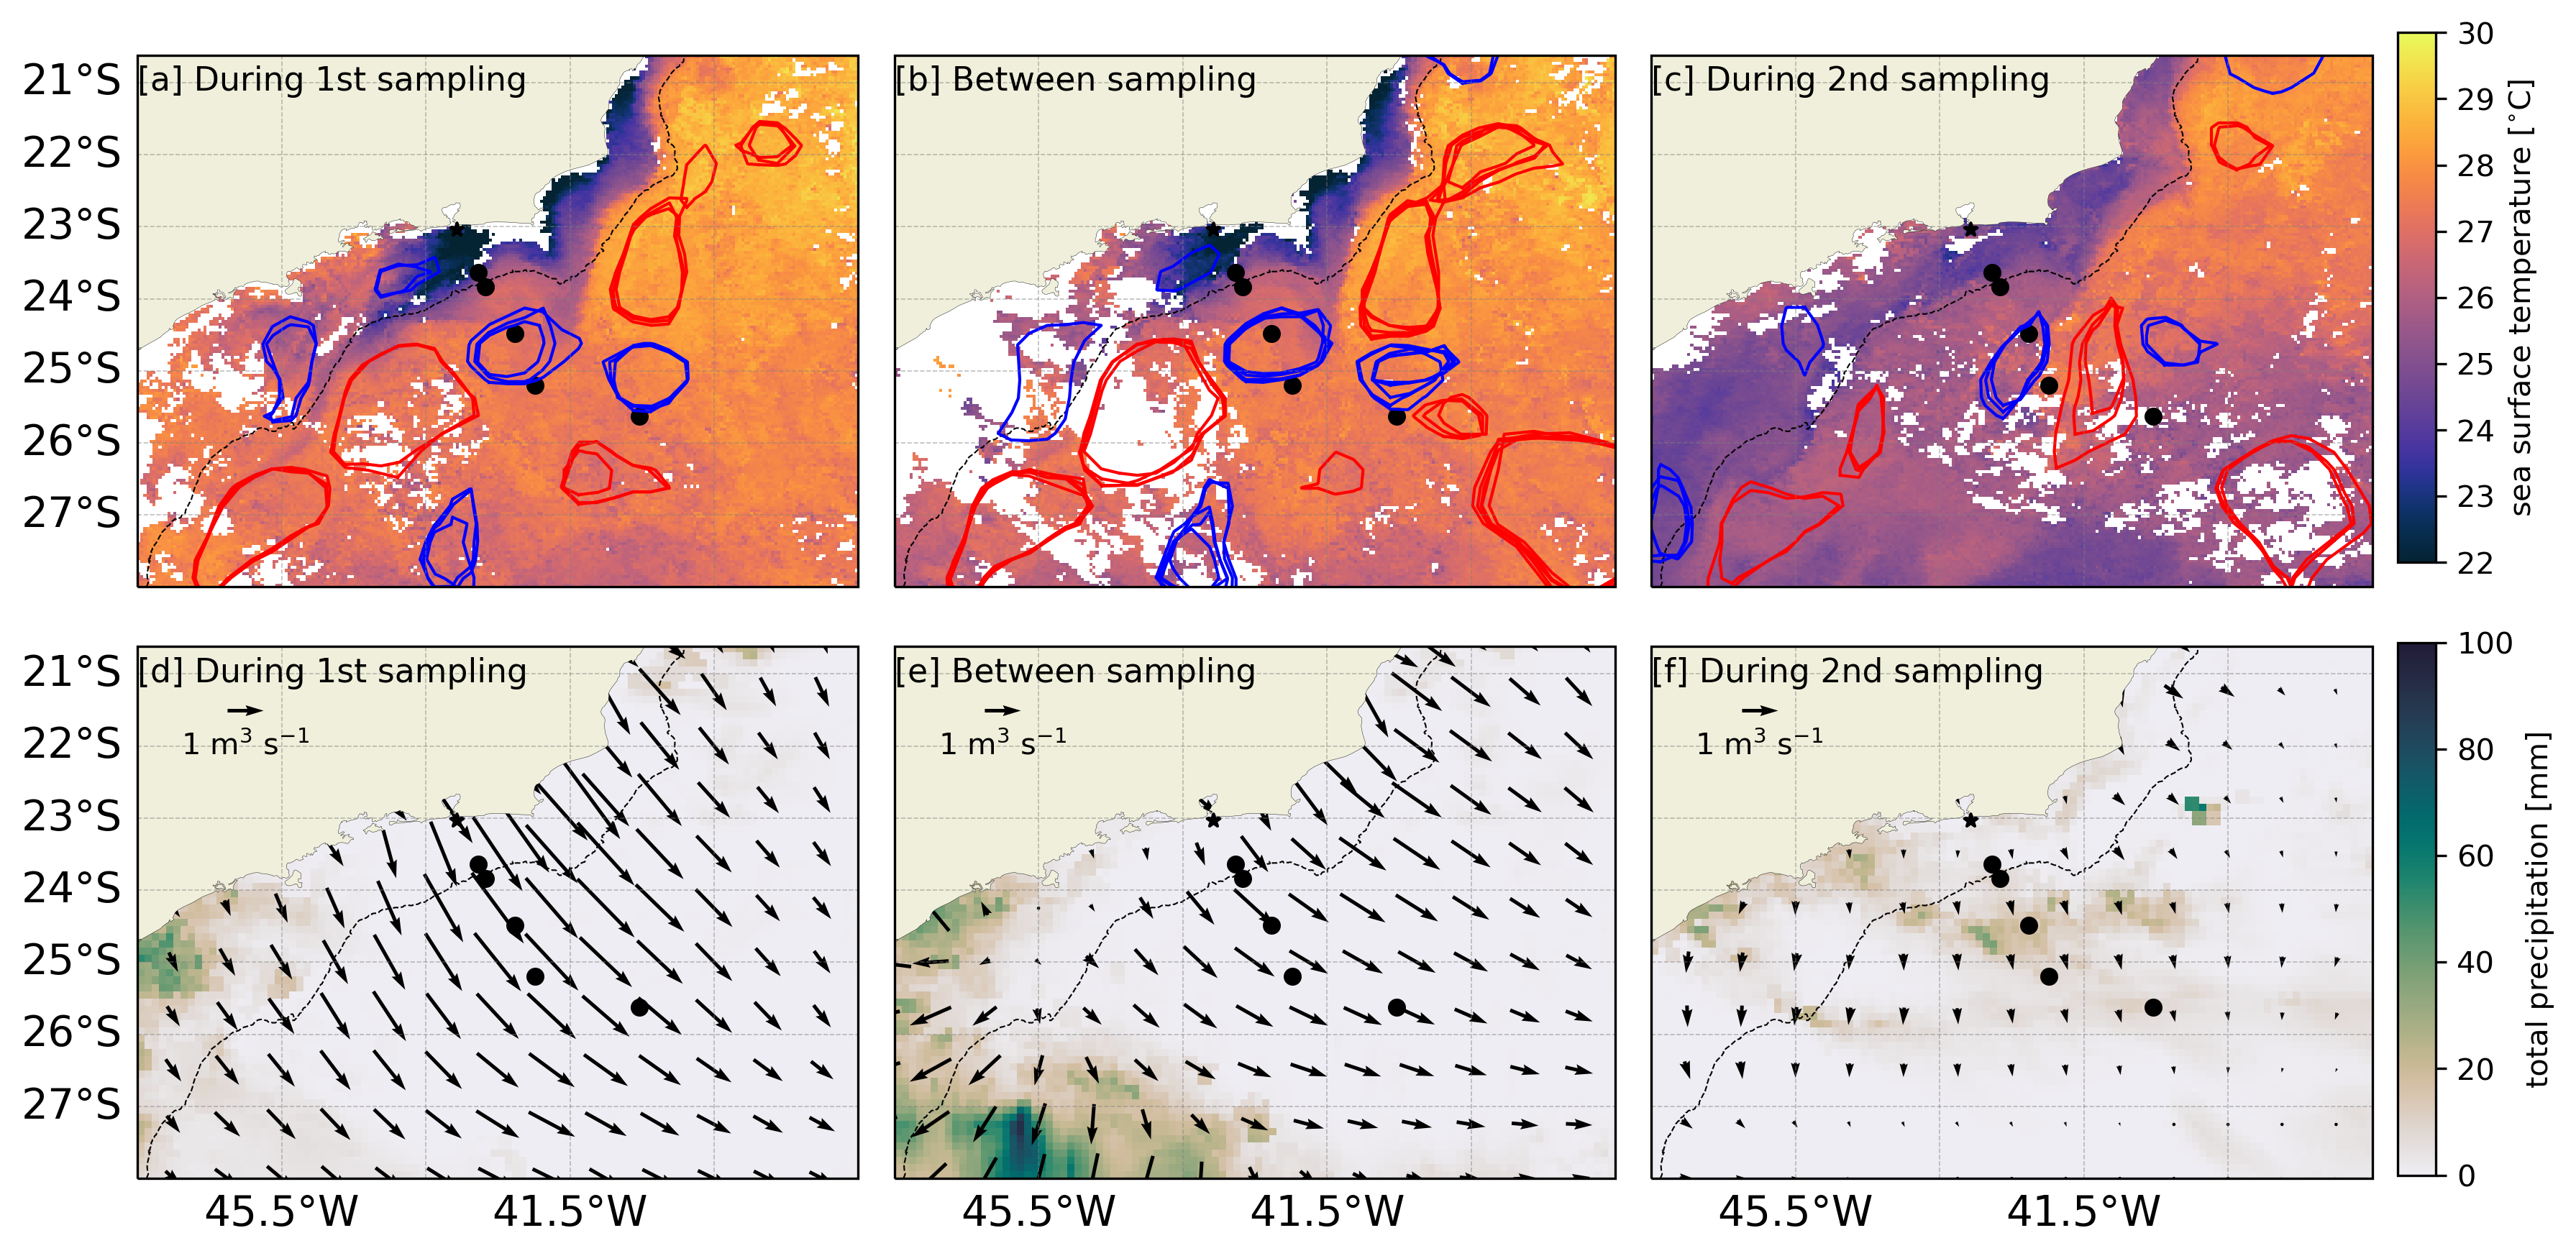
\includegraphics[width=1.\linewidth]{figures/00_manuscript_oceanographicContext.png}
    \caption{The averaged satellite-derived sea surface temperature (SST) condition are presented in the superior panels in colors (data from AVHRR), for (a) the period from 5 to 14 March (1st sampling), (b) between cruises (from 15 to 22 March) and (c) for the second sampling (23 to 28 March). These panels are superimposed by cyclonic (blue) and anticyclonic (red) eddies (obtained from Meta3.1exp DT) detected during each period. Bottom panels presents the accumulated precipitation (from the MERGE dataset) for each period with Ekman transport (calculated from ERA5 wind stress) as black vectors.}
    \label{fig:context}
\end{figure}

The weather conditions during both transects were different and may be responsible for the differences in SST. During the first cruise, the presence of upwelling-favorable winds (Figure~\ref{fig:context} d) likely reduced shelf temperatures, while weak cloud coverage favored an increase in offshore SST, contributing to the relatively larger gradient observed. During the second cruise, the passage of a frontal system a few days prior to the observations contributed to reducing the SST field throughout the domain, weakening the Ekman transport due to the reduction of wind intensity (Figure~\ref{fig:context} d).

The mesoscale signals detected in remotely sensed images were associated with the presence of \textit{$S_{max}$} during the period. For instance, SST patterns resembled a CFE signal in both cruises (Figure~\ref{fig:context}), offshore the NE-SBB (centered in, approximately, 25$^o$S and 42$^o$W). The geostrophic currents (Figure~\ref{fig:geostrophic_fields}) showed an interaction between a CFE and an Agulhas Ring (AgR), centered at approximately 24.5$^o$S and 41.5$^o$W, between February and early March (Figure~\ref{fig:geostrophic_fields} a to c). This interaction led to intense currents, reaching up to 0.6 $m s^{-1}$. Its influence over the SST field is depicted mainly as a cold water tongue at the eastern edge of the eddy (Figures~\ref{fig:context} a and b, at the same location). At the end of March, the BC splitted in two branches at 24$^o$S and 41.5$^o$W, with one branch flowing along the shelf edge, westward, and another branch flowing southwestward. This second branch meanders around a weaker CFE, and then attaches back to the shelf edge near 24$^o$S and 42.3$^o$W. The influence of the meander on the cross-shelf currents is observed on the cross-shelf geostrophic current Hovmoller along a transect following the 200-m isobath (Figure S1 a). This analysis shows two centers of intense shoreward currents occurring between January and February and during March (Figure S1 b). The projected shoreward geostrophic current occur between 24.5$^o$S and 24.0$^o$S, the same spot where the BC meander attaches back to the shelf edge. Therefore, it is expected that mesoscale activity plays an important role over the cross-shelf exchanges, in addition to upwelling-favorable winds response.

\begin{figure}[ht!]
    \centering
    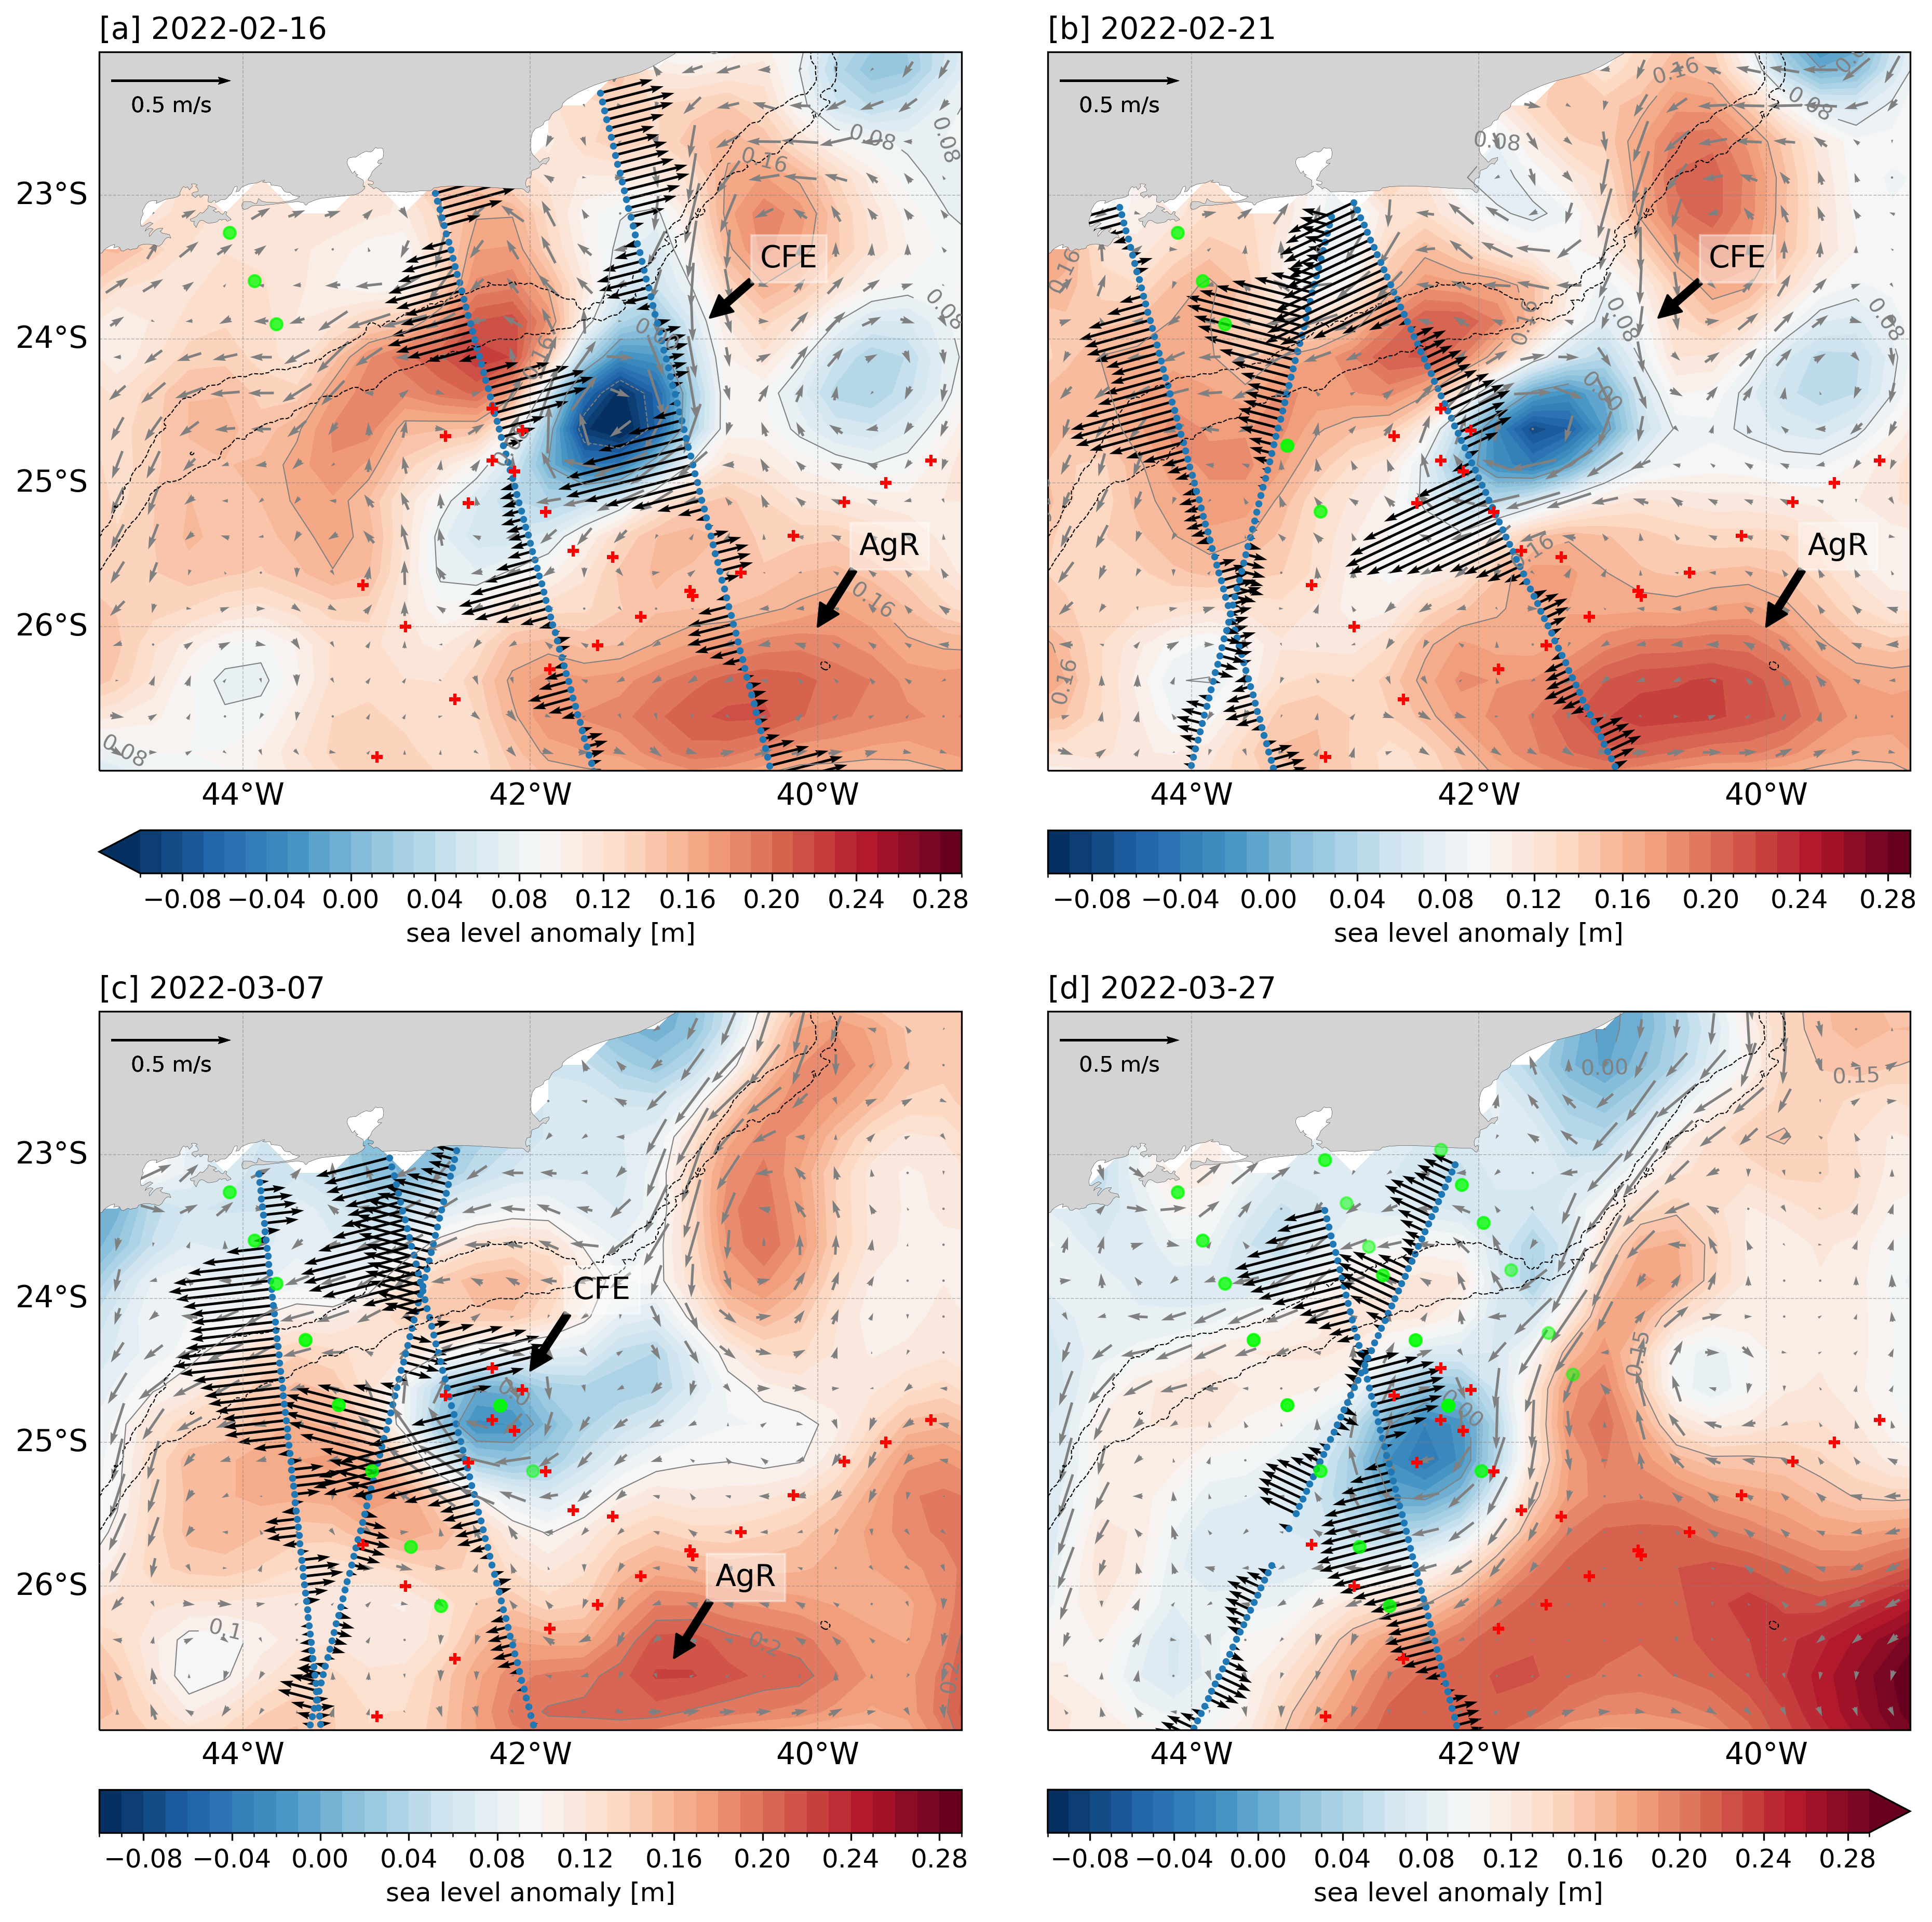
\includegraphics[width=0.8\linewidth]{figures/00_review_geostrophic_fields_with_ADT_new.png}
    \caption{Sea surface elevation anomalies (in colors and contour) from gridded AVISO for (a) 16th February, (b) 21st February, (c) 7th March and (d) 27th March. Geostrophic velocity fields overlaid the plots in gray vectors, for gridded AVISO, and computed using along-track altimeter absolute dynamic topography (ADT) in black vectors. Green markers represent locations of CTD profiles obtained by the time of each plot and red markers are the locations of the ARGO profiles. Big black arrows in (a), (b) and (c) spot the location of the Cabo Frio Eddy (CFE) and the Agulhas Ring (AgR) observed during the period.}
    \label{fig:geostrophic_fields}
\end{figure}

\subsection{Cross-shelf connectivity}
\label{subsec:cross}
The previous section presented hydrographic observations made during both cruises, revealing the presence of a \textit{$S_{max}$} intrusion (Figure~\ref{fig:cruise_transect}). To understand the origin of these structures and their entry mechanisms onto the continental shelf, we investigate the water mass characteristics and their advective velocities in this region using available ARGO profiles, a Glider dataset, and altimeter (both gridded fields and tracks) in the weeks leading to and during the cruise. We describe the results using the ARGO observations and Glider data to establish a plausible pathway indicating cross-shelf connectivity in this subsection. The two available ARGO paths chosen are shown by lines A1 (February) and A2 (February-March) in Figure~\ref{fig:study_area}. 

\textit{$S_{max}$} signals present between the open ocean and the shelf edge obtained from different measurement platforms in the weeks prior to the cruises illustrate potential connections between these environments. Two Argo profiles recorded the \textit{$S_{max}$} signals, showing consistency in their properties. In both datasets, the \textit{$S_{max}$} exhibited absolute salinity values exceeding 37.1 $g\ kg^{-1}$ at its core, with an increase of approximately 0.3 $g\ kg^{-1}$ from the surface. These signals were detected at depths ranging from 50 to 75 $m$, located below the mixed layer and between the 25 and 25.5 $kg\ m^{-3}$ isopycnals (Figure~\ref{fig:argo_alongshelf} and Figure~\ref{fig:argo_crossshelf}). The first ARGO (A1) recorded \textit{$S_{max}$} between January 20$^{th}$ and February 1$^{st}$, while during the same period, the second ARGO (A2) did not show any intrusion signal (Figure~\ref{fig:argo_alongshelf} and Figure~\ref{fig:argo_crossshelf}). A few days later, the \textit{$S_{max}$} signal was observed from February 15$^{th}$ to the end of March, while the ARGO drifted closer to the shelf edge. The similarities between these observations, particularly in the vertical position, indicate that these are the same features. According to the ARGO tracks, this signal moved towards the shelf edge, 50 and 40 days, prior to the \textit{$S_{max}$} observation over the shelf. The southwestward drift of the Argo floats limited the possibility of further analysis.

\begin{figure}[ht!]
    \centering
    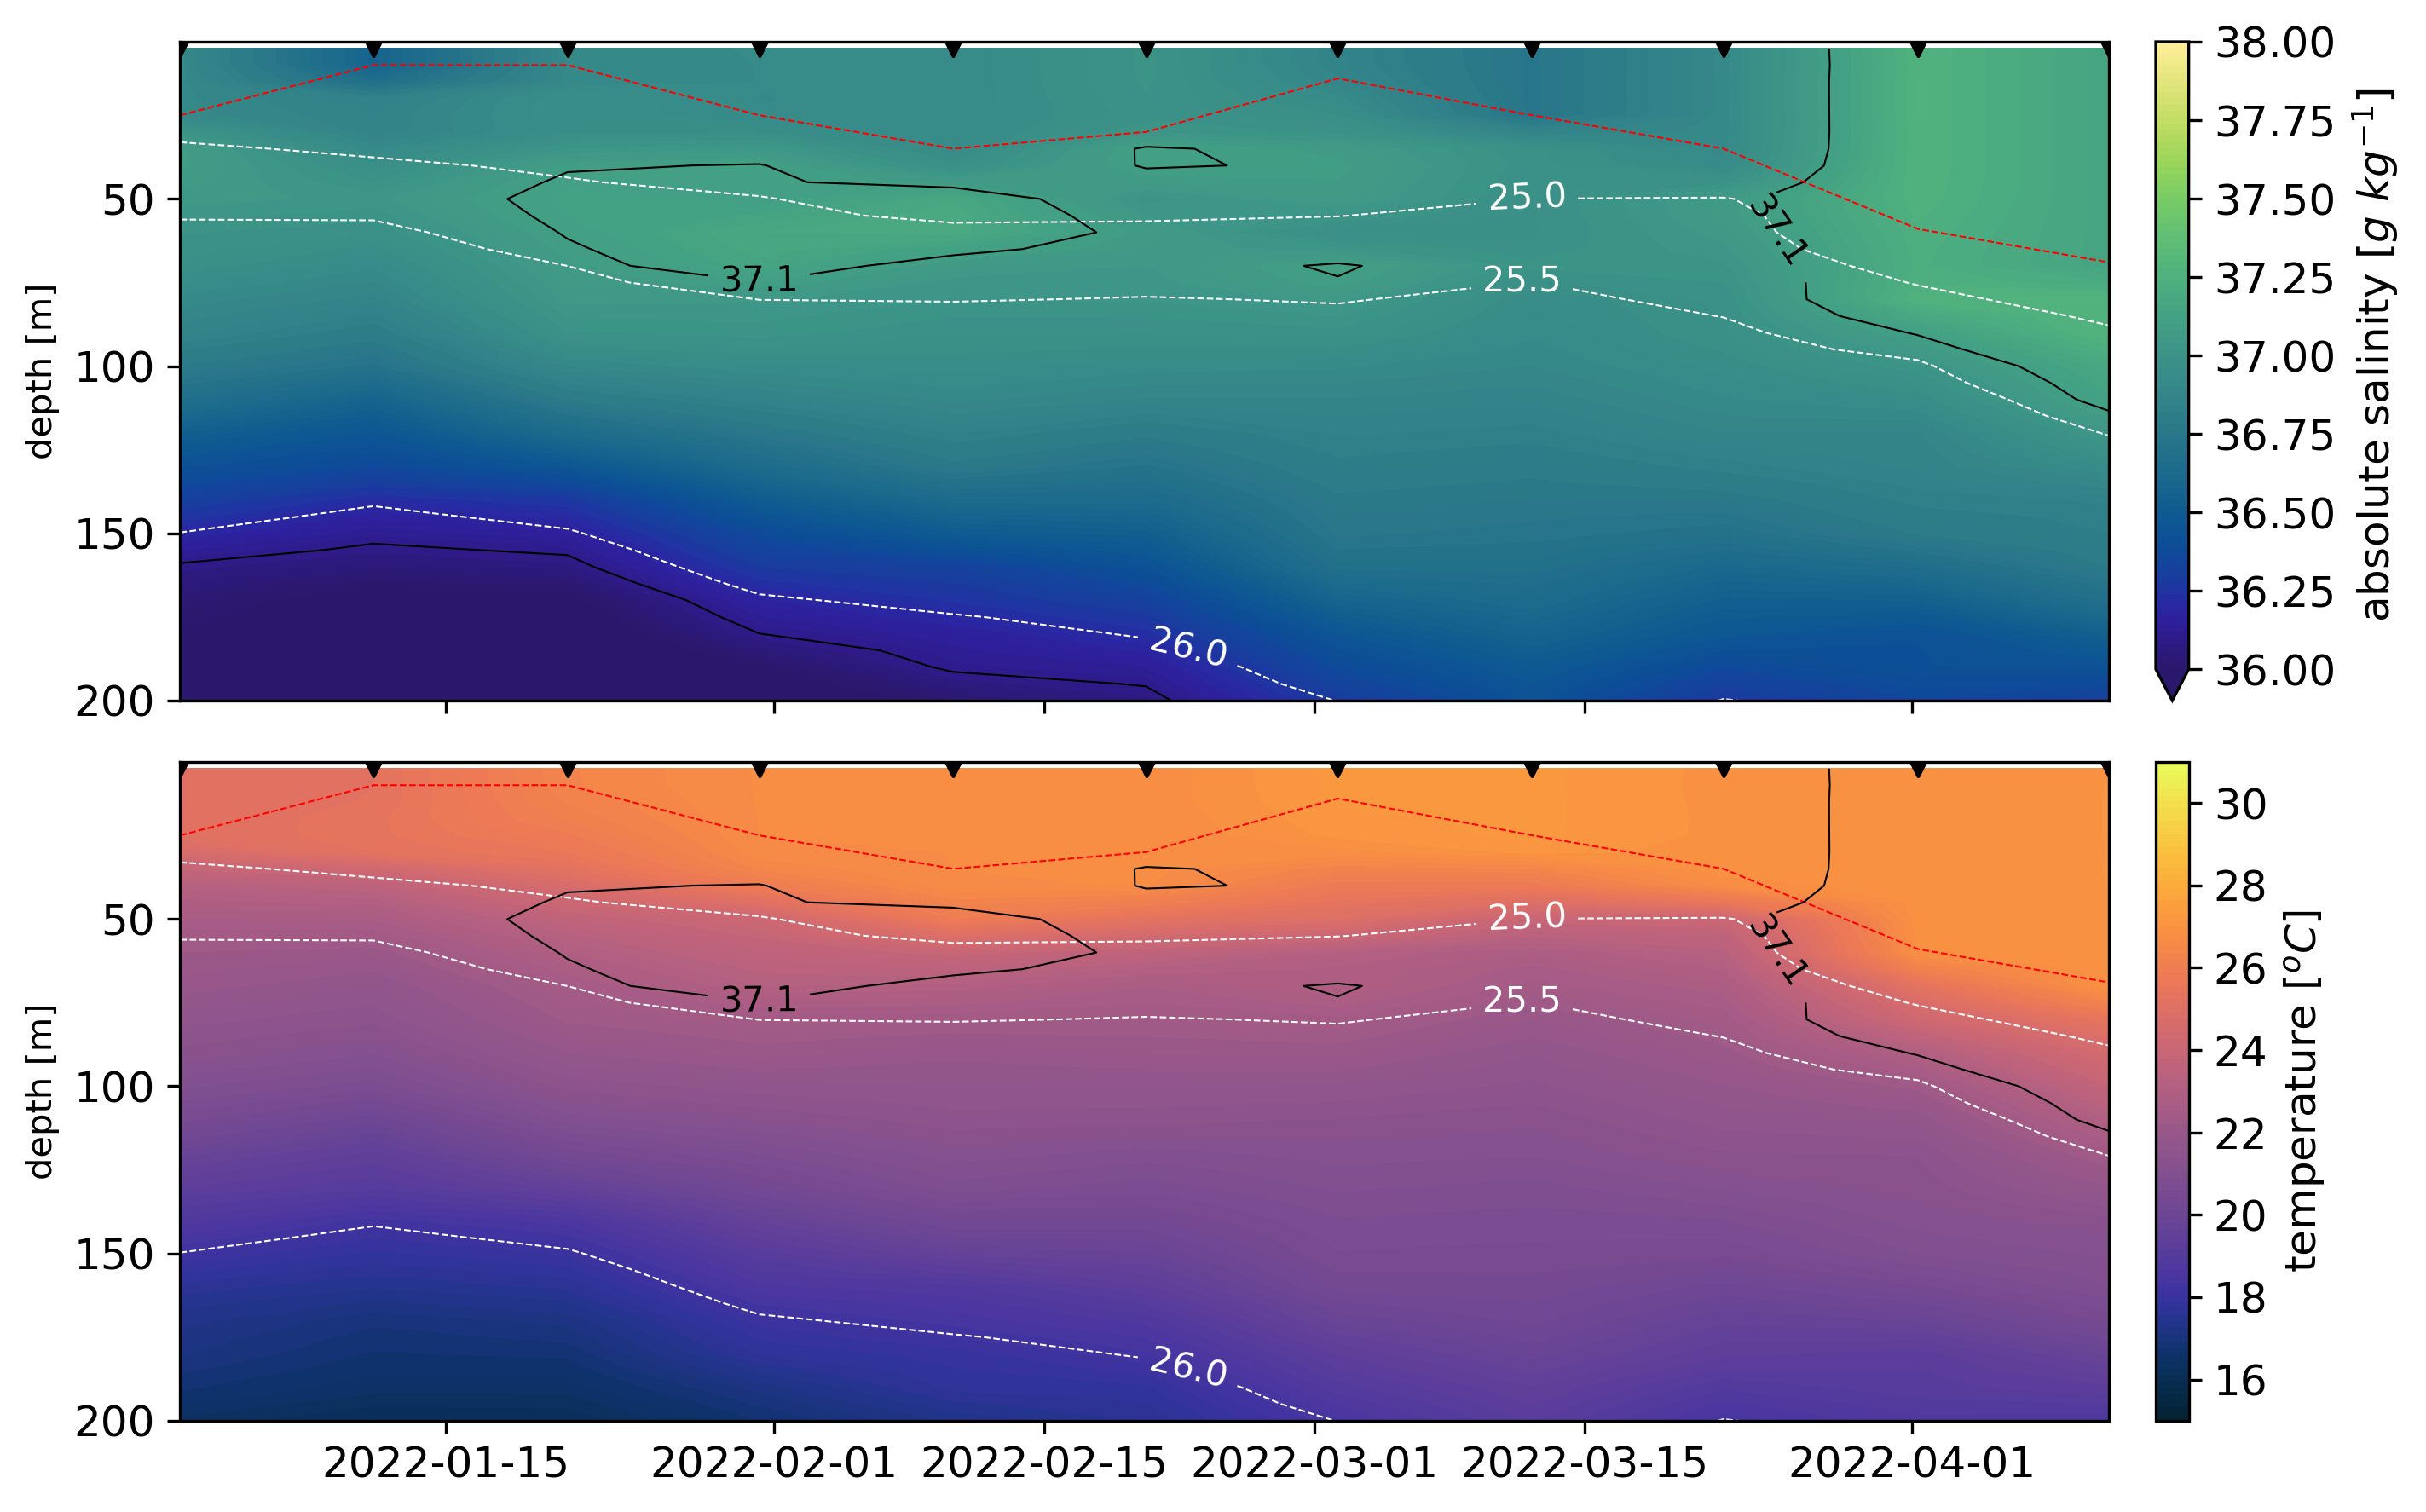
\includegraphics[width=0.8\linewidth]{figures/00_manuscript_argo_alongshelf.png}
    \caption{Transects reconstructed from ARGO profiles along line A1 in Figure~\ref{fig:study_area}  (WMO ID 3901549), for absolute salinity (top panel) and temperature (bottom panel). The black line indicates the 37.1 $g\ kg^{-1}$ isohaline, the white isopycnals for 25, 25.5 and 26 $kg\ m^{-3}$ and red dashed lines indicate the mixed layer depth, using the density criteria. The x-axis is time, while the y-axis is the depth in $m$. The path of the float is shown from northeast (left) to southwest (right) in \protect Figure~\ref{fig:study_area} as red markers}.
    \label{fig:argo_alongshelf}
\end{figure}

\begin{figure}[ht!]
    \centering
    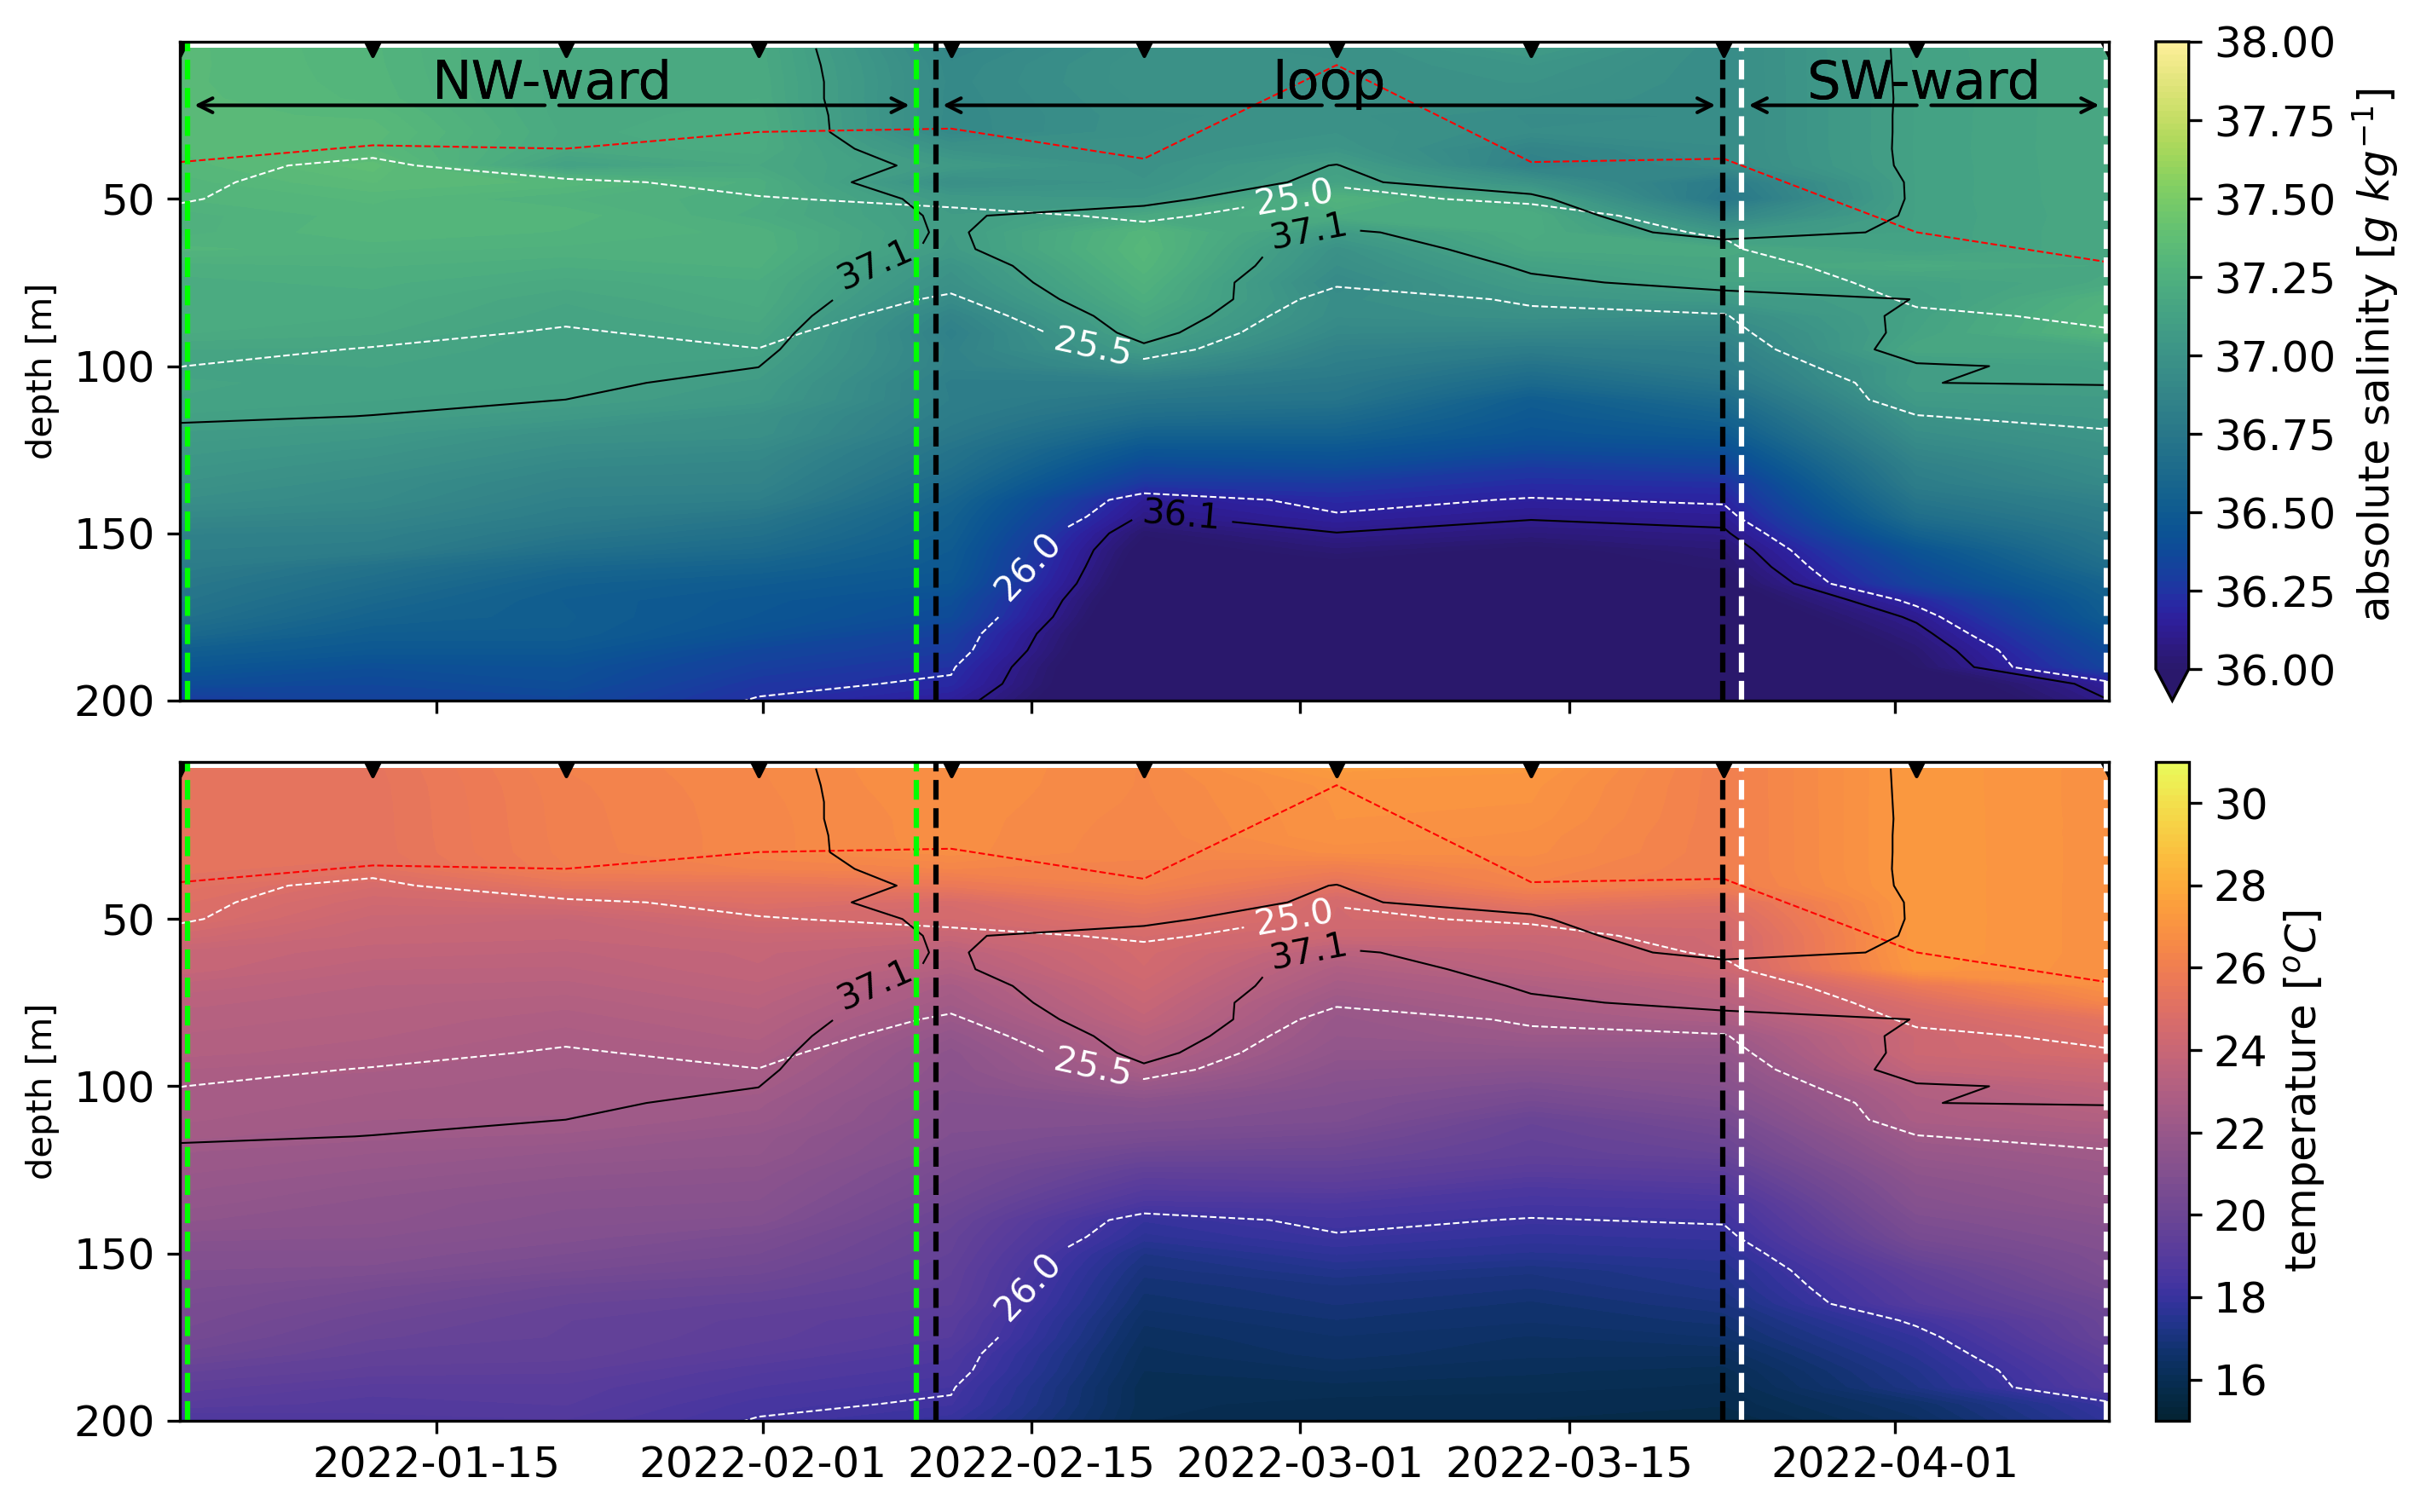
\includegraphics[width=0.8\linewidth]{figures/00_manuscript_argo_crossshelf.png}
    \caption{Same as Figure~\ref{fig:argo_alongshelf}, but for ARGO along line A2 in Figure~\ref{fig:study_area} (WMO ID 3901225) and its path from South (left) to North (right) is found in \protect Figure~\ref{fig:study_area} as black markers. The green, black and white vertical dashed lines indicates the periods according to the direction or position of the instrument during its advection (\protect Figure~\ref{fig:study_area}): }
    \label{fig:argo_crossshelf}
\end{figure}

The Slocum Glider (SG19) sampled this region during March 2022 and enabled the evaluation of the \textit{$S_{max}$} advection towards the shelf edge. In this dataset, intrusion signals similar to those detected in the Argo floats were observed (Figure~\ref{fig:glider_transect}). To describe the hydrography from the glider (Figure~\ref{fig:glider_transect}), the glider trajectory is divided in three segments for analysis: the first extends from March 3$^{rd}$ to 12$^{th}$ and represents the most offshore observations,  (Figure~\ref{fig:glider_transect} a), the second is a loop pattern followed by the glider (Figure~\ref{fig:glider_transect} b) from 13$^{th}$ to 19$^{th}$ March, while the last section with data from 22$^{th}$ to 27$^{th}$ March contains the most onshore observations (Figure~\ref{fig:glider_transect} c).

\begin{figure}[ht!]
    \centering
    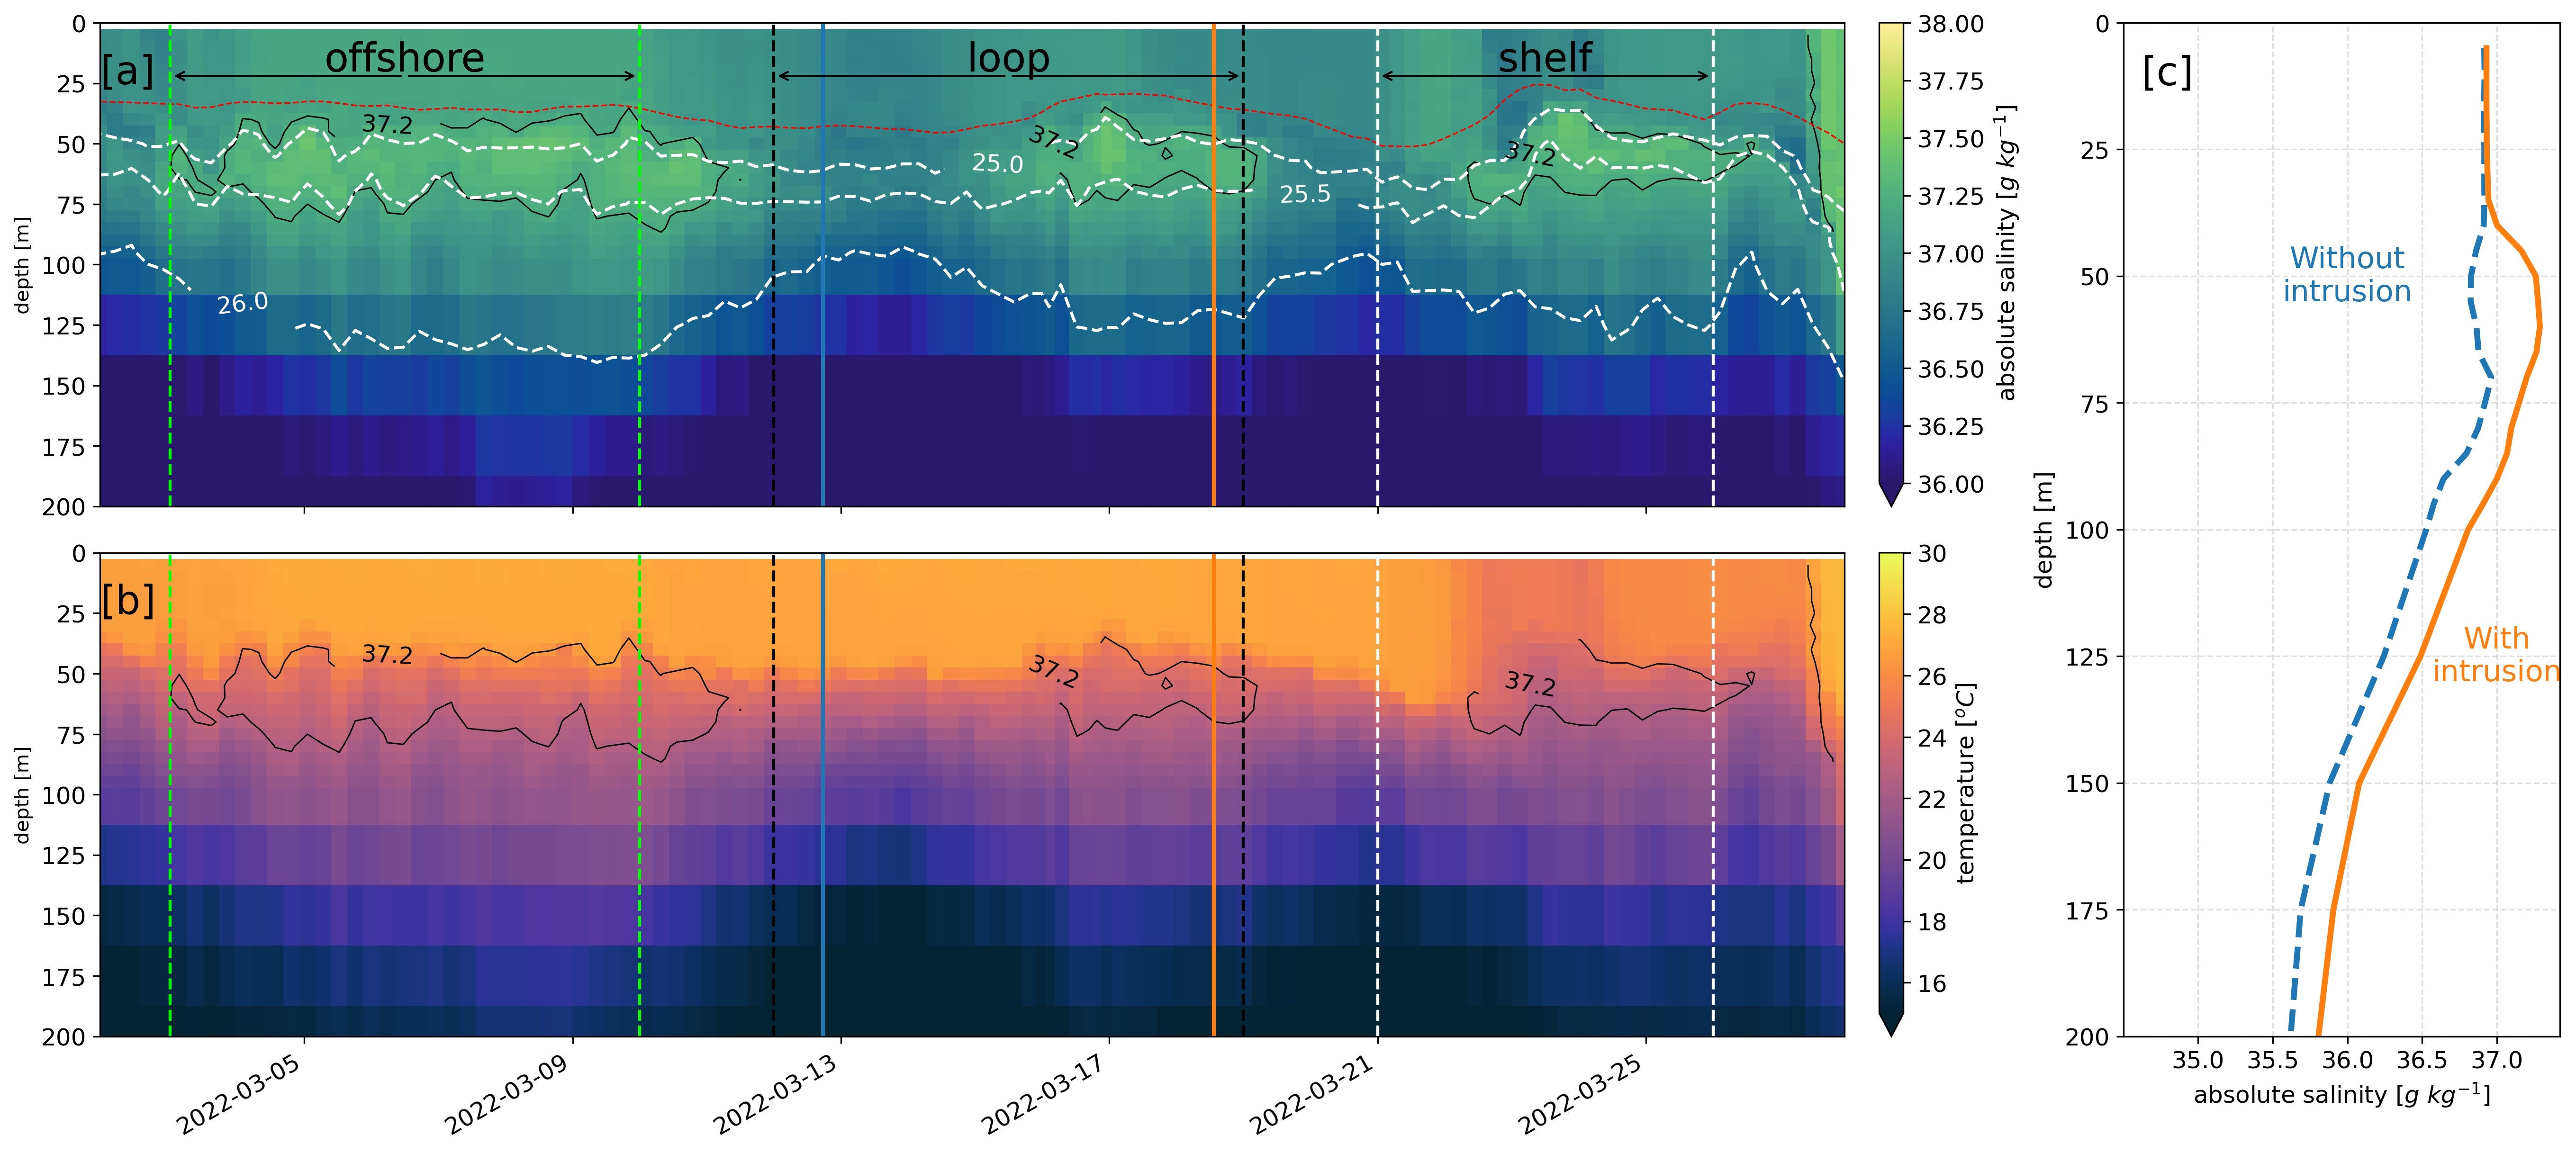
\includegraphics[width=1\linewidth]{figures/00_manuscript_glider_transect.png}
    \caption{Transects reconstructed from Slocum Glider SG19, for absolute salinity (a) and temperature (b). The black line indicates the 37.2 $g\ kg^{-1}$ isohaline, the white isopycnals for 25, 25.5 and 26 $kg\ m^{-3}$ and red dashed lines indicate the mixed layer depth, using the density criteria. The x-axis is time, while the y-axis is the depth in $m$. The path of the glider is shown in \protect Figure~\ref{fig:study_area} as a continuous black line. The green, black and white vertical dashed lines in (a) and (b) highlights periods where the \textit{$S_{max}$} was observed, while the blue and orange continuous vertical lines represents the two profiles in (c), without and with the intrusions respectively.}
    \label{fig:glider_transect}
\end{figure}

Over the entire period the first section (Figure~\ref{fig:glider_transect} a), the transect shows the presence of \textit{$S_{max}$}, covering an extension of approximately 79 $km$. After this period, the \textit{$S_{max}$} signal is absent when the glider veered towards the shelf edge and to northeast, performing the loop pattern (Figure~\ref{fig:glider_transect} b). When the glider drifted westwards, between days 15 and 20, the salinity maximum was measured once again. The glider sampled almost the same location twice in a 6-day span (Figure~\ref{fig:study_area}, zoomed map), hence, it is useful to evaluate the vertical profiles from these dives. For the first profile (Figure~\ref{fig:glider_transect} b, blue) we did not find any intrusion signal, using the \cite{silva2023inventory} methodology, but six days later the intrusion signal arrived at this location (Figure~\ref{fig:glider_transect} b, orange). The effect of \textit{$S_{max}$} increased absolute salinity from 37 $g\ kg^{-1}$ to 37.4 $g\ kg^{-1}$, between 50 and 75 $m$ depths, but also had an influence on the water column, increasing the salinity from the mixed layer depth to, at least, 200 $m$ depth, by about 0.3 $g\ kg^{-1}$. The latter portion of the glider dataset (Figure~\ref{fig:glider_transect} c) shows once again the \textit{$S_{max}$}, this time in closer proximity to the shelf edge.

\subsubsection{Water mass transformation}
\label{subsubsec:watermass}

The evaluation of specific vertical profiles from the set of hydrographic data presented allows us to describe the evolution of \textit{$S_{max}$} by advection from deep waters to the NE-SBB (Figure~\ref{fig:train_profiles}). Assuming that the same \textit{$S_{max}$} was sampled across the datasets, it is possible to track the \textit{$S_{max}$} transformation with time and relate these changes to the main hydrodynamical processes in this region, like wind or eddy-driven circulation \cite{calado2010,uchoa2023,rocha2022,silveira2023}. Figure~\ref{fig:train_profiles} shows the consecutive locations of profiles that have been traced chronologically to follow the advection of the salinity maximum intrusion from offshore to the shelf region of SBB.

In terms of water mass change throughout the profiles (Figure~\ref{fig:train_profiles} a to d), the \textit{$S_{max}$} presented salinity higher than 37 $g\ kg^{-1}$, associated with the presence of TW at the mixed layer, which is a salty and warm water mass \cite<S $\geq$ 37 $g\ kg^{-1}$ and $T$ $\geq$ 24$^o$C, >{cerda2014}, characteristic of the southwestern South Atlantic \cite{castro1998physical}. Note that the temperature in the first 3 profiles (Figure~\ref{fig:train_profiles} a to c) also shows warmer conditions, which have relevant impacts over the \textit{$S_{max}$} density. The salinity reduces to 36.5 $g\ kg^{-1}$ and temperature decreases in about 4$^o$C once over the shelf (Figure~\ref{fig:train_profiles} d and e). The drop in salinity is related to the mixing with SACW, characterized by the relatively colder waters \cite<colder than 18$^o$C, >{cerda2014}. This is possible under upwelling favorable wind conditions, in which SACW is uplifted or upwelled, decreasing the temperature and salinity at the surface levels \cite{castro1998physical,cerda2014}. The amount of information is limited and does not allow us to infer the changes between the first and the second profiles. However, these hydrographic conditions reveal the influence of local processes in the vertical position \textit{$S_{max}$} and the density associated with the maximum salinity.

\begin{figure}[ht!]
    \centering
    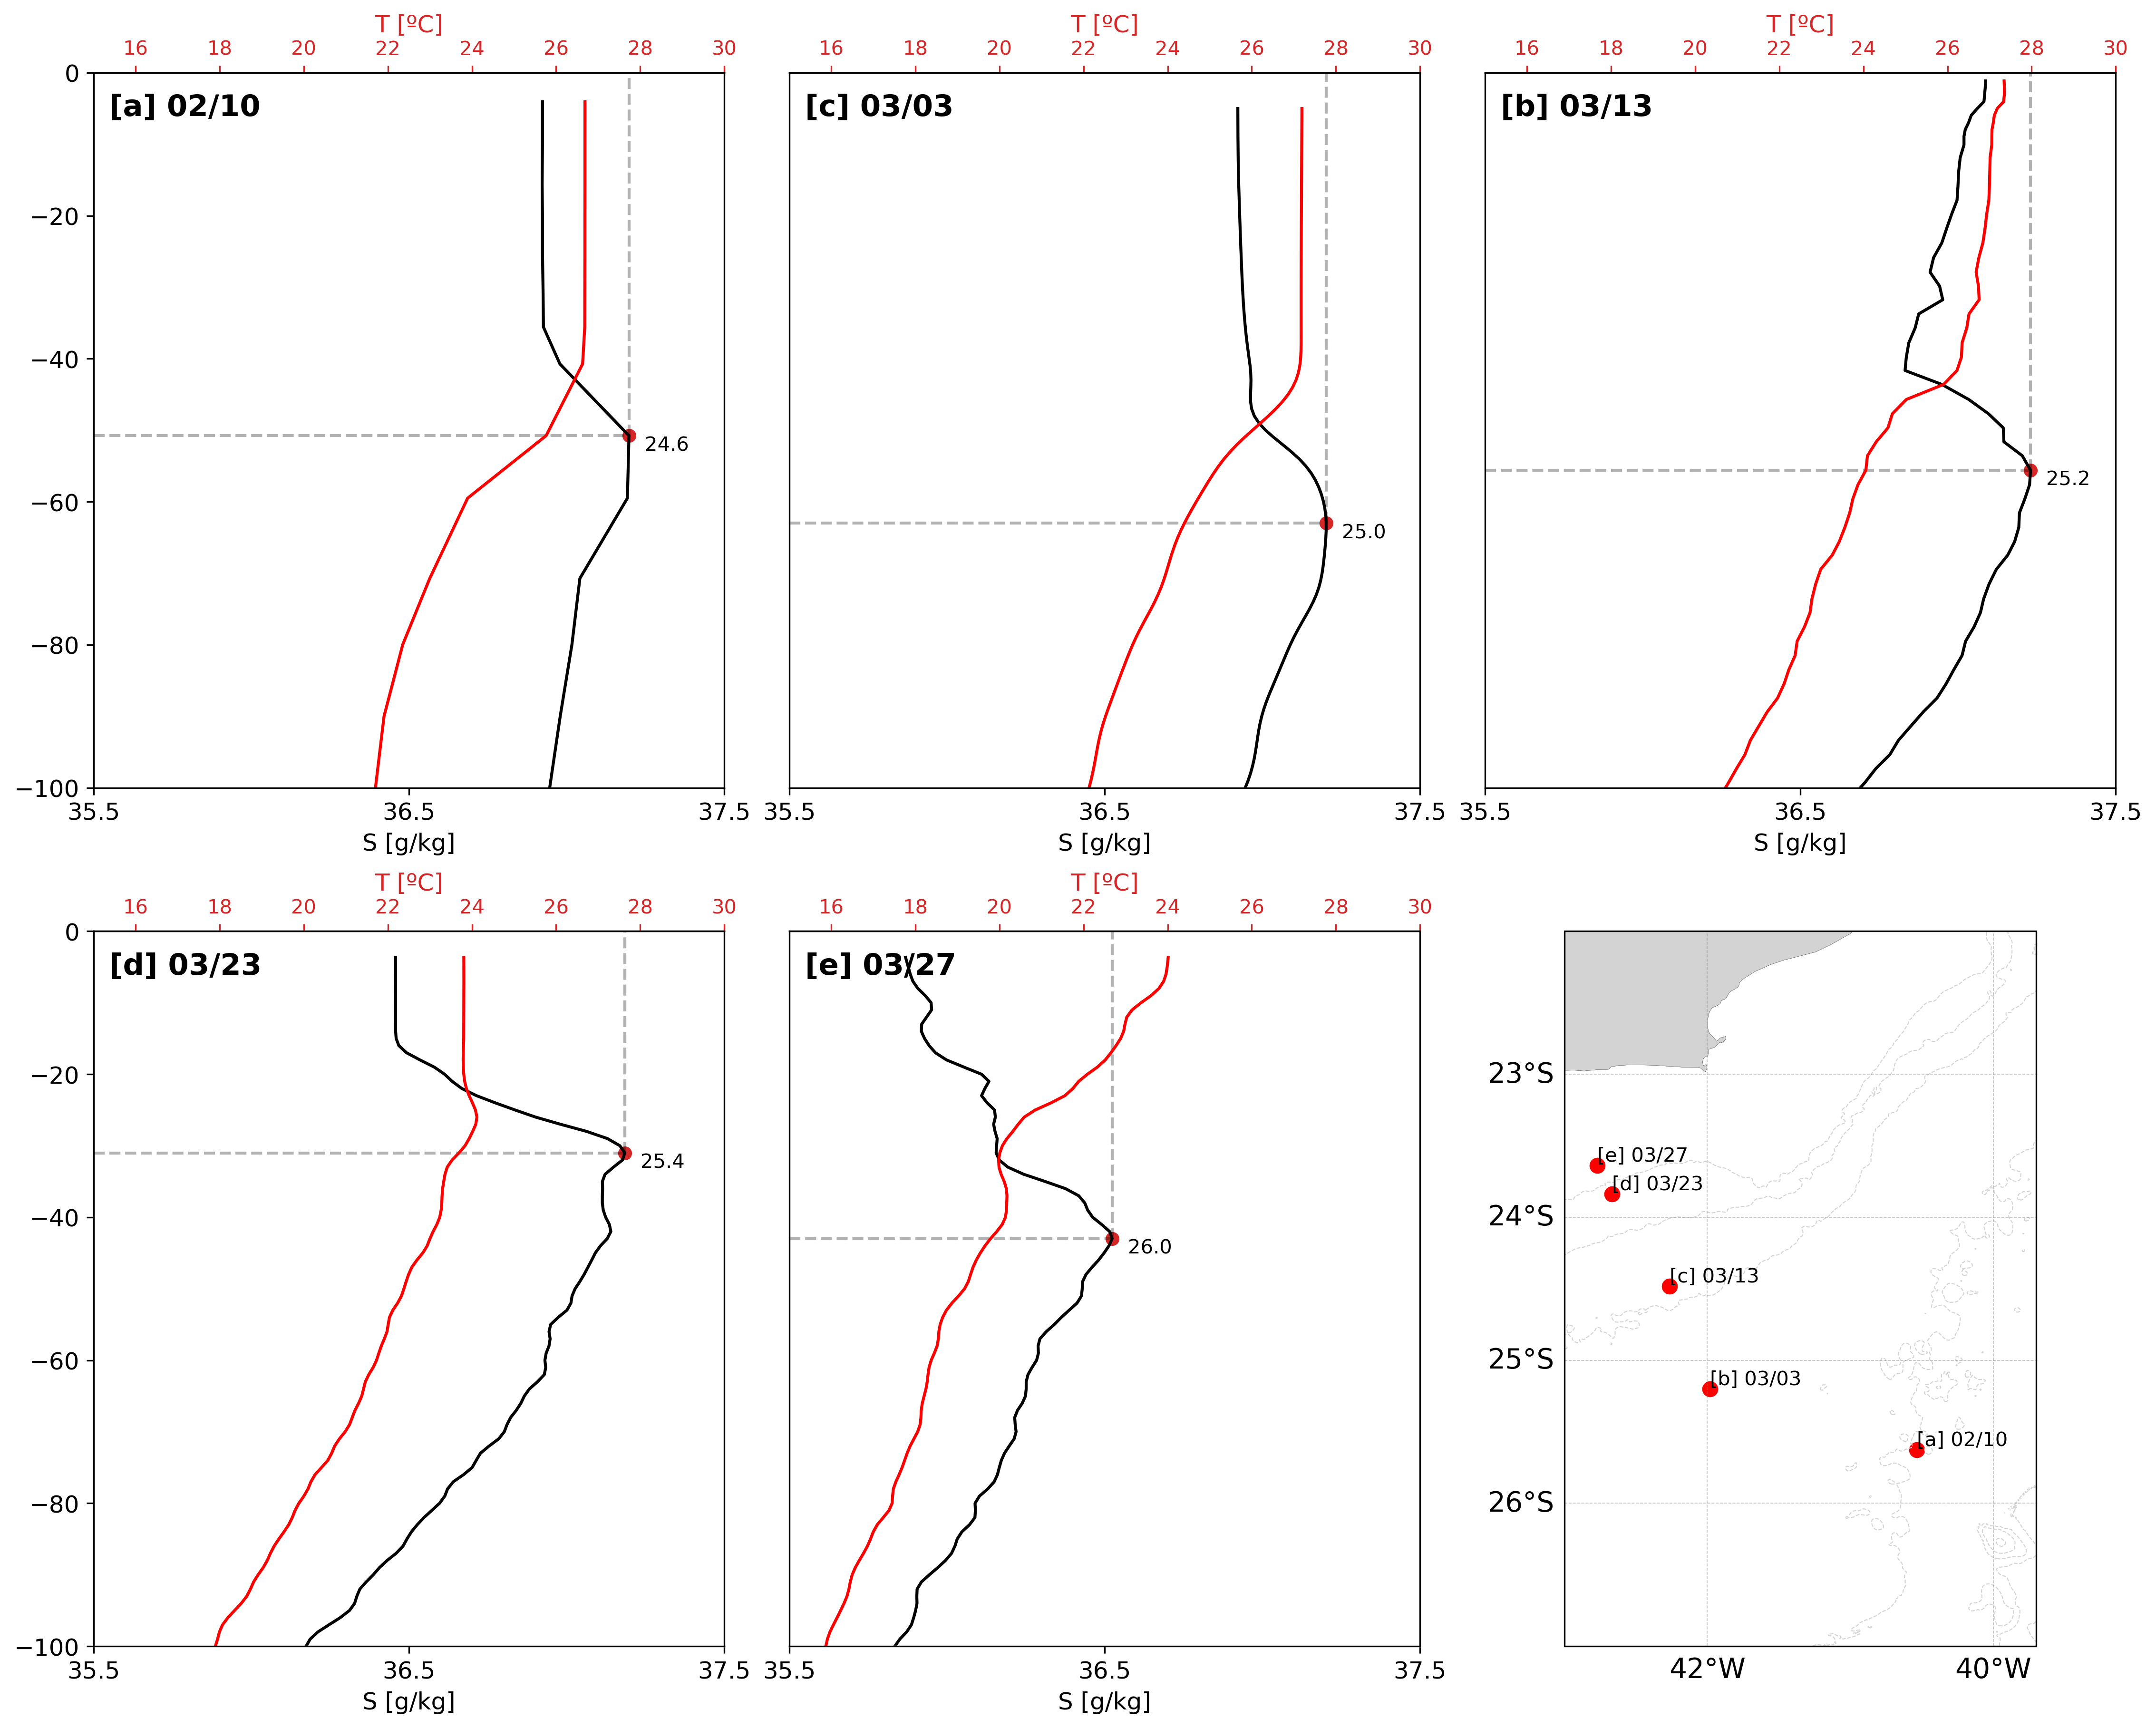
\includegraphics[width=0.8\linewidth]{figures/00_manuscript_train_profiles_new.png}
    \caption{Selected sequence of absolute salinity (black) and temperature (red) profiles with \textit{$S_{max}$} detected by the algorithm used by \protect\citeA{silva2023inventory}. Each vertical profile, from a to e, presents the depth of the \textit{$S_{max}$} as red marker along its potential density (in $kg\ m^{-3}$). In (f) there is the geographical position of each profile, along with their dates for reference.}
    \label{fig:train_profiles}
\end{figure}

Following \citeA{silva2023inventory}, who reported that \textit{$S_{max}$} are most often located around the 25.5 $kg \ m^{-3}$ isopycnal, we compared GLORYS salinity patterns at 50 m depth with those along this isopycnal layer. The isopycnal layer exhibits higher salinity values on the continental shelf compared to the 50-m layer, whereas the 50-m layer shows an overall higher salinity across the entire domain compared to the isopycnal field. Note that the GLORYS output is given in practical salinity (psu), and no further analysis was performed on this dataset, such as converting to absolute salinity ($g\ kg^{-1}$). Thus, they differ from the observational data set presented earlier. The salinity fields temporal evolution is available in the Supplementary Video V1. 

Between February 18 and March 3, the 50 m layer fields exhibit a \textit{$S_{max}$} intrusion (S $>$ 37 psu) originating from the east (Supplementary Video V1, left). This salty feature appears to be advected by a mushroom-shaped mesoscale structure and progresses westward until it dissipates when it reaches the continental shelf break around March 3. In contrast, the isopycnal layer fields show an increase in salinity over the shelf region, between Guanabara Bay and Cabo Frio, after March 3 (Supplementary Video V1, left). This salinity increase merges with saltier waters advected from north along the shelf, resulting in an expanded saline area between Guanabara Bay and Cabo Frio. After a few days, waters in this region are gradually replaced by relatively fresher waters near the coast, probably associated with coastal upwelling processes.

\subsection{Lagrangian Pathways}
\label{subsec:lagpath}

Based on the GLORYS analysis on the previous section, \textit{$S_{max}$} found at a fixed depth (e.g., 50-m layer) disappeared as it advected toward the shelf break. In addition, the isopycnal surfaces show saltier waters found within the shelf, suggesting that \textit{$S_{max}$} might enter the shelf following a specific isopycnal, as suggested by \citeA{silva2023inventory}. In order to evaluate these pathwats, we performed two backward Lagrangian experiments, considering (i) LBPI: a full three-dimensional experiment, using GLORYS as a hydrodynamical field and releasing particles at a given depth (50 m) and (ii) LBPII: an experiment using velocities extracted from GLORYS but at a specific isopycnal (25.5 kg m$^{-3}$), thus considered a two-dimensional experiment. In all experiments, 100 particles were released within a 1$^o$ degree box around a center launching point: for both LBPI and LBPII at 42.77$^o$W and 23.64$^o$S (where \textit{$S_{max}$} were last seen in our observational dataset). The particles were launched on 27 March, also in agreement with the last observation of \textit{$S_{max}$}. Table~\ref{tab:lagrangian_experiments} summarizes the setup of the Lagrangian experiment. 

\begin{table}[ht!]
\caption{Summary of Lagrangian experiments performed, along with seeding center and depth, number of particles launched distributed over a 1$^o$ squared box and date of release. This location, depth and date are related to the last vertical profiles in which \textit{$S_{max}$} was detected. LPB1 and LPB2 are backpropagation experiments using the 3D GLORYS12V1 hydrodynamical field and the 25.5 kg m$^{-3}$ isopycnal velocity, respectively.}
\label{tab:lagrangian_experiments}
\begin{tabular}{c c c c c c}
\hline
\textbf{experiment} & \textbf{center} & \textbf{depth [m]} & \textbf{seeded particles} & \textbf{date} & \textbf{{[}B/F{]}} \\
\hline
LBP1                  & 42.77$^o$W; 23.64$^o$S & 50                     & 100          & 2022-03-27 & B    \\ 
LPB2                  & 42.77$^o$W; 23.64$^o$S & -                      & 100         & 2022-03-27 & B     \\ 
\hline
\end{tabular}
\end{table}

The simulated particle transport pathways reveal significant cross-shelf components that can be advected westward either through a meandering pathway offshore of NE-SBB or via along-shelf advection over the 200 m isobath, both occurring within approximately 40 days (Figure~\ref{fig:lagrangian_analysis}a). These results indicate two potential advection pathways for \textit{$S_{max}$}: (1) a more probable cross-shelf pathway, originating from the east, and (2) the along-isobath pathway, originating from the north.

The cross-shelf pathway represents the highest probability, accounting for 30$\%$ of the particles seeded on the shelf (LBPI, Figure~\ref{fig:lagrangian_analysis} a). It presents a meandering-like shape, swirling in the along shelf direction, but transporting particles effectively in the cross-shelf direction. There is a hotspot of particles centered at 42$^o$W and 25$^o$S, where they do not present a concise pathway, but instead an accumulation, although a main path is still distinguishable. After 40 days, the particles reach deeper regions, crossing isobaths during advection, reaching the 200 $m$ isobath to almost 4000 $m$ isobath. This Lagrangian analysis result presents a better fit with the selected vertical profiles used to understand the transformation of the water mass (Figure~\ref{fig:train_profiles}), as observed by the red dots in Figure~\ref{fig:lagrangian_analysis} a.

\begin{figure}[ht!]
    \centering
    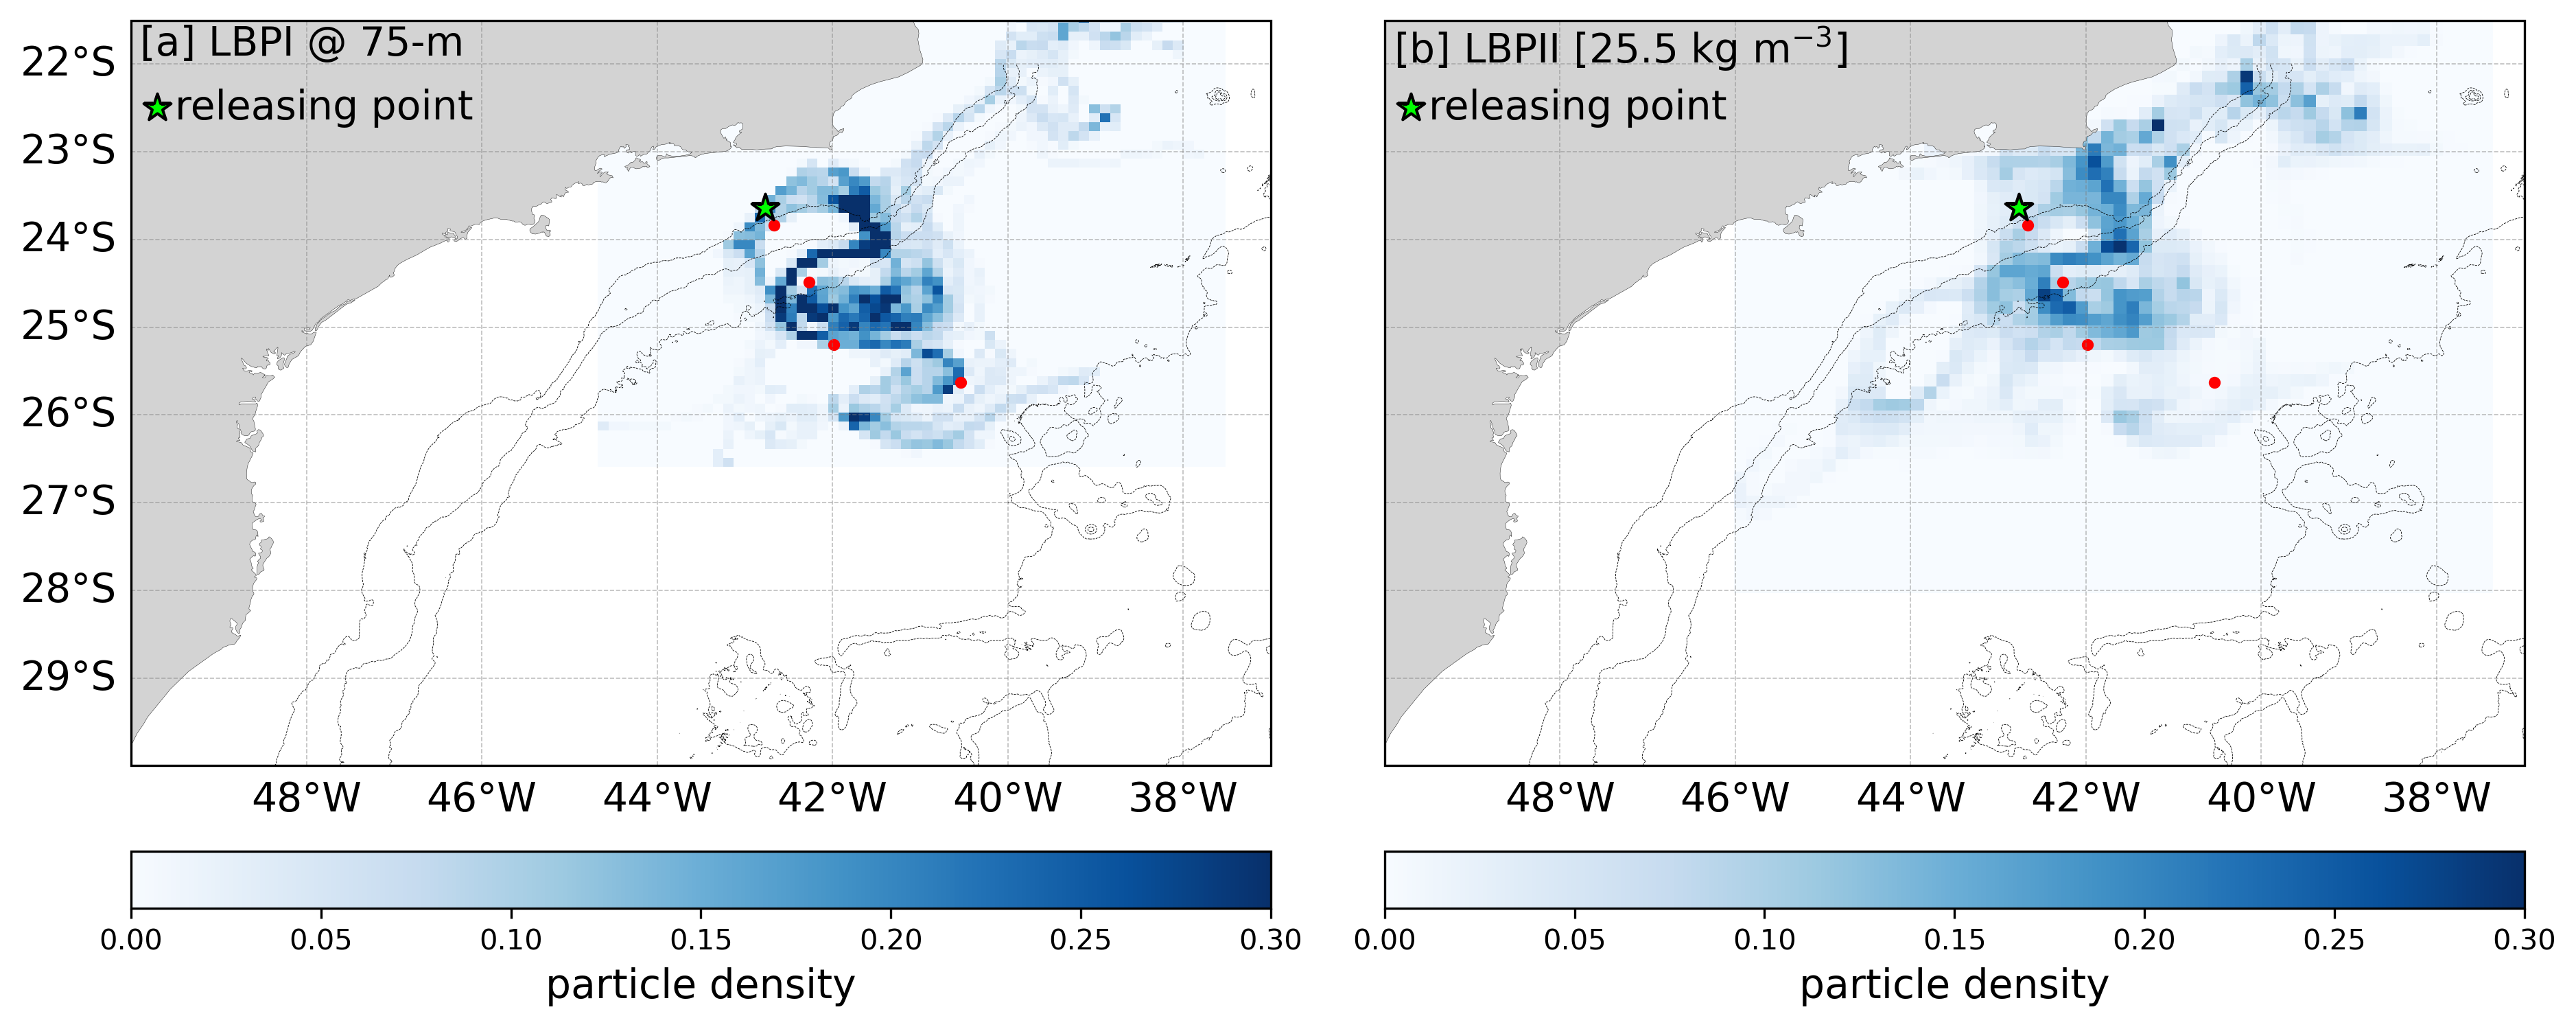
\includegraphics[width=1\linewidth]{figures/00_manuscript_lagrangian_analysis.png}
    \caption{Time integrated particles concentration on (a) the 3D GLORYS12V1 and (b) the isopycnal surface velocities backpropagation experiments with release at the last \textit{$S_{max}$} observed on 27th March over the shelf at 50-m depth. The red markers indicates the location of the sequence of profiles from \protect Figure~\ref{fig:train_profiles}. Green stars on each panel represent the releasing location, better described in Table~\ref{tab:lagrangian_experiments}.}
    \label{fig:lagrangian_analysis}
\end{figure}

In Figure~\ref{fig:lagrangian_analysis} a, a reduced lateral extent of particle presence was observed on the continental shelf, near the releasing point, which does not fully explain the mechanism by which \textit{$S_{max}$} enters the shelf. To further investigate this cross-shelf a similar backtracking experiment was conducted considering velocities on isopycnal surfaces. We assumed that \textit{$S_{max}$} was advected predominantly along the 25.5 kg m$^{-3}$ isopycnal, based on the analysis by \citeA{silva2023inventory}. The results of this experiment (LBPII, Figure~\ref{fig:lagrangian_analysis} b) show a pattern broadly similar to the previous one, revealing two primary pathways, one from the north and another from the east, which transport particles along the shelf break and across the shelf, respectively. In particular, this second experiment shows a larger area with particles within the shelf, particularly between Cabo de São Tomé and Guanabara Bay, distinguishing it from the first experiment. Moreover, in this second analysis, particles continue southwestwards, reaching the SBB central area (43.5$^0$W; 25.5$^0$S), where their accumulation suggests anticyclonic trapping \cite{silveira2023}.

Although the east source seems to be the most probable origin of March 2022 \textit{$S_{max}$}, as shown by the cross-shelf pathway, a secondary source was identified from the backpropagation analysis. The along-isobath pathway brings particles from the Tubarão Bight (28.25$^o$S), north of the region of interest (Figure~\ref{fig:lagrangian_analysis} a), transporting particles following the isobaths. However, in the region of interest, the along-isobath merges with the cross-shelf pathway, and it is not possible to separate one from the other. 

\subsection{Ekman Transport on the Shelf}
\label{sub:ekman}

The surface Ekman transport ($T_{Ek}$), calculated from wind stress, is presented in Figure~\ref{fig:context} as vectors. It shows that throughout the first observational cruise, $T_{Ek}$ was predominantly towards offshelf (Figure~\ref{fig:context} d), due to constant northeasterly winds, from the South Atlantic Subtropical High \cite<SASH, >{stech1990estudo}, generating an offshelf Ekman Transport of approximately 80 $m^3\ s^{-1}$. Winds from SASH has an average intensity of 10 $m\ s^{-1}$ \cite{pimenta2019brazil}, with a lower frequency of cold fronts \cite{stech1990estudo}, its persistence drives significant cross-shelf exchanges, pushing water offshore and by mass conservation cold and nutrient rich waters (SACW) upwells or uplift nearshore. It results in coastal upwelling such as the one observed during the first transect, which also generates a cross-shelf SST gradient (Figure~\ref{fig:context} a). Between both samplings, the wind patterns changed and intensified, associated with a cold front passage that inverted the wind direction \cite{stech1990estudo}. Not only did it affect the sea surface by changing the input of momentum, but also the incident solar radiation due to an increase in cloud coverage, which subsequently reduced the SST (Figure~\ref{fig:context} b). The wind inversion was not persistent enough to generate an onshelf surface $T_{Ek}$ (not shown), resulting only in relatively weaker offshelf $T_{Ek}$, reducing from 50 $m^3\ s^{-1}$ between cruises (Figure~\ref{fig:context} e) to 20 $m^3\ s^{-1}$ in the second cruise (Figure~\ref{fig:context} f).

Onshore transport occurs at depth in response to offshore Ekman transport at the surface, either near the bottom or in midwater \cite{LentzChapman2004}. During the analyzed period, the onshelf transport over the shelf edge was expected to be above the bottom Ekman layer, i.e., in subsurface levels, as given by the slope Burger number ($Bu$) higher than 1 \cite{LentzChapman2004} as presented in Table~\ref{tab:burger_number}.

\begin{table}[ht!]
\caption{Summary of topographic gradient ($\alpha$), Buoyancy Frequency ($N^2$) and Burger number ($Bu$, Equation~\ref{eq:burger}) computed for specific CTD profiles extracted from SANAGU14 and SANAGU15 campaings.}
\label{tab:burger_number}
\centering
\begin{tabular}{c c c c}
\hline
\textbf{Vertical profile} & \textbf{$\alpha$} & \textbf{$N^2 [s^{-1}]$} & \textbf{$Bu$} \\
\hline
        G4 & $23 \times 10^{-3}$ & $5.96 \times 10^{-5}$ & 9.15 \\
        G4' & $23 \times 10^{-3}$ & $4.65 \times 10^{-5}$ & 7.14 \\
        H4 & $11 \times 10^{-3}$ & $5.32 \times 10^{-5}$ & 2.16 \\
\hline
\multicolumn{2}{l}{$\alpha$ and $Bu$ are dimensionless numbers.}
\end{tabular}
\end{table}

\section{Discussion}
\label{section:discussion}

During the campaign in March 2022, multiple Salinity Maximum (\textit{$S_{max}$}) intrusions were observed off the Northeastern South Brazil Bight (NE-SBB). We found these signals were associated with the local stratification, occurring at the pycnocline, mainly between the 25 and 25.5 $kg\ m^{-3}$ isopycnals, and below the mixed layer (Figures~\ref{fig:cruise_transect},~\ref{fig:argo_alongshelf},~\ref{fig:argo_crossshelf},~\ref{fig:glider_transect}). The vertical extents of the salinity maximum intrusions occur between the 50 and 75 $m$ depths, resulting in an average thickness of 25 $m$, consistent with the climatological thickness of 30 m for the \textit{$S_{max}$} intrusions in the NE-SBB \cite{silva2023inventory}. The salinity anomaly of 0.3 $g\ kg^{-1}$ spans between the summer (0.59 $g\ kg^{-1}$) and winter (0.34 $g\ kg^{-1}$) of the same climatology \cite{silva2023inventory}. 
However, the maximum salinity values observed were higher than those described by \citeA{silva2023inventory} over the shelf, i.e waters saltier than 37.1 $g\ kg^{-1}$ in observations over the open ocean and 36 $g\ kg^{-1}$ over the shelf. These differences were expected, as \textit{$S_{max}$} during this period occurred offshore, beyond the reach of continental freshwater runoff in the NE-SBB \cite{cerda2014,castro2014summer}. Thus, SACW may contribute to a reduction in the maximum salinity near the surface through coastal or eddy-induced upwelling processes \cite{calado2010,cerda2014,castro2014summer}. \textit{$S_{max}$} SBB intrusions exhibit characteristics similar to those observed in the Northeast United States shelf \cite<Middle Atlantic Bight or MAB, >{Lentz2003}. These intrusions are typically associated with subsurface salinity maxima, most prominent during summer at mid-depths, with vertical extents ranging from 20 to 30 m. The formation and persistence of these features are likely associated with a combination of advective and double-diffusive processes \cite{Lentz2003,gawarkiewicz2022increasing,silva2023inventory,gawarkiewicz2025mapping}. In addition, particularly in the MAB, \textit{$S_{max}$} intrusions are becoming more frequent since the 2000's, associated with an increase in Warm Core Rings \cite{gangopadhyay2019observed,silver2023increased}, and penetrating larger distances shoreward \cite{gawarkiewicz2022increasing} relative to previous studies.  MAB \textit{$S_{max}$} intrusions are formed from the interaction between anticyclonic mesoscale eddies characterized by warm core rings, with shelf break \cite{silver2023increased}. In the SBB case, the cyclones, particularly the CFE, appear as a possible driving mechanism of \textit{$S_{max}$} intrusions into the shelf, similar to the ones found in Australia \cite{Malan2020}.

Our investigation demonstrates the advection of \textit{$S_{max}$} intrusions from the deeper ocean to the NE-SBB, predominantly via cross-shelf pathways, but also through along-shelf pathways, depending on mesoscale dynamics (Figure~\ref{fig:lagrangian_analysis}). Figure~\ref{fig:schematic} summarizes the key pathways and components found in the absolute dynamic topography of AVISO and Lagrangian analysis schematically. The observational dataset reveals that intrusion signals were found below the mixed layer in all observations (Section~\ref{sec:smax_structure}) which, in a first approximation, could be defined as the maximum depth where high-frequency atmospheric processes play a role in the hydrodynamics near the surface \cite{giunta2022ocean}. Thus, it is reasonable to assume that the mesoscale dynamical processes were responsible for the advection of the \textit{$S_{max}$} signal towards the shelf edge. One of the curious questions unresolved from this data set is the offshore occurrence of the \textit{$S_{max}$}. It is possible that the \textit{$S_{max}$} was originally formed within the Brazil Current system or propagating saltier eddies \cite<much like warm core rings in the North Atlantic, >{silver2023increased} and then advected in the offshore regions of the SBB. In fact, the backpropagation Lagrangian analysis indicates that in both pathways, the most probable origin of \textit{$S_{max}$} is located north of the NE-SBB, from where it is advected poleward by local mesoscale dynamics (Figure~\ref{fig:lagrangian_analysis}) supporting this idea.

During February and March 2022, the dataset presented here suggests the cross-shelf pathway as the main source of salty water mass at that time (Figure~\ref{fig:lagrangian_analysis} a) and can be obtained from two different paths that meet at an offshore junction location near 41.5$^0$W; 25$^0$S: a cross-shelf and another alongshelf pathways (Figure~\ref{fig:lagrangian_analysis}). The cross-shelf pathway could be driven by a northern limb of an incoming Agulhas Ring \cite<AgR, >{bernardo2025trapping}, see Figure~\ref{fig:geostrophic_fields} a for an example and Figure~\ref{fig:schematic} red solid line, advecting \textit{$S_{max}$} towards the shelf. During its advection, the \textit{$S_{max}$} achieves an unstable region, where the BC meanders, often necking off Cabo Frio Eddies \cite<CFE, >{rocha2022,uchoa2023,silveira2023}. In the confluence formed by the pairing of an AgR and CFE, it appears that \textit{$S_{max}$} were captured by the BC meander (see Figure~\ref{fig:geostrophic_fields} a for an example and Figure~\ref{fig:schematic} dark blue solid line) and advected further towards the shelf edge. Geostrophic field analysis (Figure~\ref{fig:geostrophic_fields}) suggests that the second half of the cross-shelf pathway is driven by the BC meander. The along-shelf pathway contribution is not negligible and represents a secondary source of \textit{$S_{max}$}, coming from the North (Figures~\ref{fig:lagrangian_analysis} a and c). This pathway resembles the BC non meandering state (Figure~\ref{fig:schematic} dashed blue line), flowing along the isobaths (Figure~\ref{fig:geostrophic_fields} c). The BC eventually becomes unstable and starts to meander, growing at an average rate of $0.1\ day^{-1}$ \cite<see Figure 3 in>{silveira2023}, until it reaches a state of necking off a CFE \cite{uchoa2023}. In this case, the \textit{$S_{max}$} advection will present a cross-shelf pattern, similar to the meander centered at 24.5$^o$S and 42$^o$W in Figure~\ref{fig:schematic}. 

\begin{figure}[ht!]
    \centering
    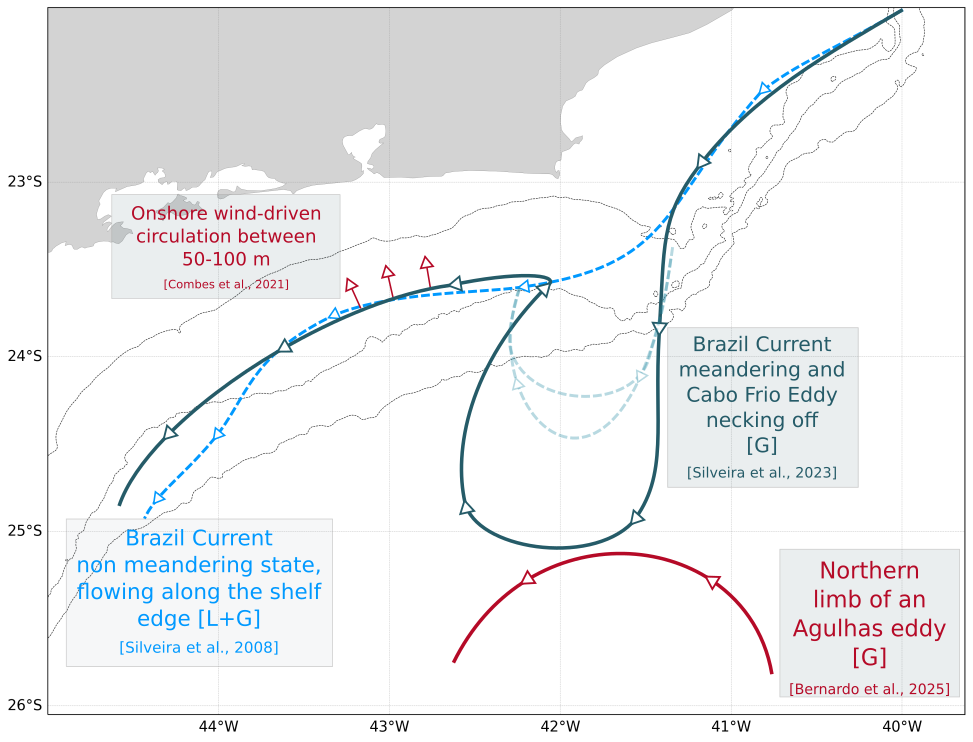
\includegraphics[width=1\linewidth]{figures/pathways_schematics_structure.png}
    \caption{Schematic flow field summarizing the three pathways scenarios of Salinity Maximum intrusions, obtained from the jointly analysis of the geostrophic fields (G, Figure~\ref{fig:geostrophic_fields}) and lagrangian outputs (L, Figure~\ref{fig:lagrangian_analysis}). The cross-shelf pathway is a combination of the northern limb of an Agulhas eddy (red) and the meandering state of the Brazil Current (BC, dark blue), while the along-shelf edge pathway is given in dashed light blue, resembling the non-meandering state of the BC.}
    \label{fig:schematic}
\end{figure}

\citeA{silva2023inventory} reported that \textit{$S_{max}$} in the SBB region are found between the 24 and 26 kg m$^{-3}$ isopycnals. These findings suggest that analyses based on a single fixed depth level - such as those presented in Supplementary Video V1 (left) - or fixed depth velocity fields (e.g. Figure~\ref{fig:lagrangian_analysis} a) are insufficient for accurately capturing \textit{$S_{max}$} occurrences. Examination of isopycnal surfaces (Supplementary Video V1, right) reveals a distinct core of saltier waters along the SBB. This structure is consistent with the results of the Lagrangian analysis, which indicates a higher concentration of particles on the shelf (Figure~\ref{fig:lagrangian_analysis} b) compared to the fixed-depth experiment (Figure~\ref{fig:lagrangian_analysis} a). Although the precise mechanisms responsible for transporting \textit{$S_{max}$} onto the shelf are uncertain, cross-shelf transport ageostrophic processes probably play a significant role, since geostrophic currents are restricted to flow along isobaths \cite{brink2016,chen2022mesoscale}. For instance, mesoscale eddies have been shown to enhance shelf-slope exchanges in various regions \cite{mizobata2006, Malan2020, rautenbach2023, eshghi2023impact}, and may similarly influence \textit{$S_{max}$} dynamics in the SBB.

In the northeastern SBB, wind-driven cross-shelf exchanges have been documented between 50 and 100 m depth \cite{combes2021circulation}, facilitating onshelf advection under northeasterly (upwelling-favorable) wind conditions that were present during the period of interest (see Ekman transport in Figure~\ref{fig:context} d to f). The slope Burger number ($Bu$, Table~\ref{tab:burger_number}) supports this interpretation, with values exceeding one indicating a preferential mid-depth cross-shelf pathway during observational campaigns \cite{LentzChapman2004}. These values suggest that stratification and topographic slope play a central role in constraining the vertical structure of \textit{$S_{max}$} intrusions. A higher $Bu$, resulting from stronger stratification or steeper topographic slopes, generates a counter-flux at shallower or intermediate depths in response to surface Ekman transport, thus confining intrusions to these layers. In contrast, lower $Bu$ values, associated with weaker stratification or smooth topography, drive the counter-flux within the bottom layer, generating deeper intrusions. From a historical perspective, the depth and thickness of \textit{$S_{max}$} also respond to changes in the stratification of the water column \cite{silva2023inventory}. Under higher stratification, intrusions are typically shallower and thinner, primarily due to the presence of denser water masses beneath the intrusion, such as the South Atlantic Central Water (SACW). In contrast, lower stratification allows for deeper and thicker intrusions.

Our analysis suggests the interaction between the Cabo Frio eddy (CFE) and the Agulhas Ring (AgR) advect the \textit{$S_{max}$} towards the shelf edge, while the shoreward wind-driven circulation (Ekman dynamics) is responsible by pushing \textit{$S_{max}$} intro the shelf, leading to a \textit{$S_{max}$} intrusion. Despite these insights, the available observational dataset is insufficient to fully resolve the interactions among these processes. This highlights the need for high-resolution numerical simulations to evaluate their relative contributions under varying forcing scenarios \cite<e.g.,>{wang2011,paloczy2016,Chen2019}.

\section{Concluding Remarks}
\label{section:concluding}

In this study, we present the first observational evidence of remotely advected mid-depth Salinity Maximum (\textit{$S_{max}$}) intrusions in the Northeastern South Brazil Bight (NE-SBB). Using a multi-platform observational dataset, we tracked the pathway of \textit{$S_{max}$} from eastern locations off the NE-SBB to the continental shelf in this region. Our findings indicate that oceanic \textit{$S_{max}$} is consistent with those observed over the shelf \cite{silva2023inventory}, characterized by waters saltier than 37 $g\ kg^{-1}$ and occurring between 50 and 100 m depth. Backpropagation Lagrangian results indicate the origin of \textit{$S_{max}$} being northeast of the study region.

A key result of this study identifies the Cabo Frio Eddy (CFE) as the main mechanism advecting \textit{$S_{max}$} towards the shelf, describing a cross-shelf pathway. Once at the shelf break, Ekman transport associated with upwelling-favoable winds act as the main process pushing \textit{$S_{max}$} further onto the shelf. In addition to the cross-shelf pathway, our analysis found two secondary processes: (i) the enhancement of the advection process by the interaction between the CFE and an incoming Agulhas Ring (AgR) and (ii) an southwestwar alongshelf pathway, resembling a non-meandering Brazil Current regime, advecting \textit{$S_{max}$} directly from their source.

Our results shed light on the origins and pathways of \textit{$S_{max}$}, a poorly understood phenomenon in the SBB. Recognizing these intrusions of warm, salty waters is essential for advancing our understanding of the Cabo Frio upwelling system. Moreover, under climate change scenarios, further studies in the NE-SBB are required to evaluate how \textit{$S_{max}$} dynamics may influence the thermodynamics of the continental shelf.

%%%%%%%%%%%%%%%%%%%%%%%%%%%%%%%%%%%%%%%%%%%%%%%
%
% DATA SECTION and ACKNOWLEDGMENTS
%
%%%%%%%%%%%%%%%%%%%%%%%%%%%%%%%%%%%%%%%%%%%%%%%

\section*{Open Research Section}

The CTD casts from the SANAGU campaign \cite{moreira2023multidisciplinary}, belong to Petrobras and are not accessible to the public or research community. The ARGO profiles were obtained on April 2023 from the \textit{Institu Français de Recherche pour l'Explotation de la Mer} (IFREMER), via ARGOPY package \cite<\url{https://joss.theoj.org/papers/10.21105/joss.02425}, >{Maze2020}. The Slocum Glider SG19 dataset is not accessible to the public or research community, but it is possible to request access through ProjetoAzul at \url{http://www.projetoazul.eco.br/}. GLORYS data is available from EU Copernicus Marine Service at \url{https://doi.org/10.48670/moi-00016} \cite{jean2021glorys}. ERA5 output is available from the Copernicus Climate Change Service at \url{https://doi.org/10.24381/cds.adbb2d47} \cite{hersbach2018era5}. The bathymetry data were downloaded from GEBCO 2019 \cite{weatherall2015new}. The altimeter dataset and derivative products from them were processed by SSALTO/DUACS and distributed by AVISO+ (\url{https://www.aviso.altimetry.fr}) with support from the \textit{Centre national d'études spatiales} (CNES).  The precipitation dataset from MERGE were obtained on April 2023, from the National Institute on Spatial Research (or INPE in Brazilian portuguese) website (\url{https://ftp.cptec.inpe.br/modelos/tempo/MERGE/GPM/DAILY/}). The sea surface temperature were obtained from the National Centers for Environmental Information (NCEI), via their website (\url{https://www.ncei.noaa.gov/data/oceans/pathfinder/Version5.3/L3C/}). This work used the Gibbs-Seawater Oceanographic Toolbox with the python package GSW \cite{mcdougall2011gsw}, CTD data were processed with Python-CTD \cite{Fernandes2014}, multi-dimensional data were handled using Xarray \cite{xarray2017}, data analysis were performed with NumPy \cite{numpy2020} and data visualization was made with Matplotlib \cite{Hunter2007Matplotlib}. All scripts used to reproduce the figures and analysis in this manuscript are available at \url{https://zenodo.org/records/12735815}.

\acknowledgments
We thank Petróleo Brasileiro S.A. (PETROBRAS) for their permission to use and display the proprietary data from Santos Project – Santos Basin Environmental Characterization – for this paper. The authors would like to thank all the organizations for making the dataset used in this research available and the School of Marine Science and Technology/University of Massachusetts Dartmouth (SMAST/UMassD) for their support during this research. Danilo A. Silva and Dalton K. Sasaki acknowledge financial support from PETROBRAS (Santos Project, 2018/00068-8), Marcelo Dottori acknowledges support from the Fundação de Amparo à Pesquisa do Estado de São Paulo (FAPESP 2010/05124-1) and Ilson Carlos Almeida da Silveira acknowledges support from CNPq (Project HIDROSAN I, 405593/2021-0) and FAPESP (Project HIDROSAN II, 2021/13124-6). We also thank the reviewers for their valuable suggestions and comments, which considerably improved the quality of this article.

%%%%%%%%%%%%%%%%%%%%%%%%%%%%%%%%%%%%%%%%%%%%%%%
% REFERENCES and BIBLIOGRAPHY
\bibliography{references}
% \bibliography{<name of your .bib file>} don't specify the file extension
% don't specify bibliographystyle
%
%%%%%%%%%%%%%%%%%%%%%%%%%%%%%%%%%%%%%%%%%%%%%%%

\end{document}




More Information and Advice:

%%%%%%%%%%%%%%%%%%%%%%%%%%%%%%%%%%%%%%%%%%%%%%%
%
%  SECTION HEADS
%
%%%%%%%%%%%%%%%%%%%%%%%%%%%%%%%%%%%%%%%%%%%%%%%

% Capitalize the first letter of each word (except for
% prepositions, conjunctions, and articles that are
% three or fewer letters).

% AGU follows standard outline style; therefore, there cannot be a section 1 without
% a section 2, or a section 2.3.1 without a section 2.3.2.
% Please make sure your section numbers are balanced.
% ---------------
% Level 1 head
%
% Use the \section{} command to identify level 1 heads;
% type the appropriate head wording between the curly
% brackets, as shown below.
%
%An example:
%\section{Level 1 Head: Introduction}
%
% ---------------
% Level 2 head
%
% Use the \subsection{} command to identify level 2 heads.
%An example:
%\subsection{Level 2 Head}
%
% ---------------
% Level 3 head
%
% Use the \subsubsection{} command to identify level 3 heads
%An example:
%\subsubsection{Level 3 Head}
%
%---------------
% Level 4 head
%
% Use the \subsubsubsection{} command to identify level 3 heads
% An example:
%\subsubsubsection{Level 4 Head} An example.
%
%%%%%%%%%%%%%%%%%%%%%%%%%%%%%%%%%%%%%%%%%%%%%%%
%
%  IN-TEXT LISTS
%
%%%%%%%%%%%%%%%%%%%%%%%%%%%%%%%%%%%%%%%%%%%%%%%
%
% Do not use bulleted lists; enumerated lists are okay.
% \begin{enumerate}
% \item
% \item
% \item
% \end{enumerate}
%
%%%%%%%%%%%%%%%%%%%%%%%%%%%%%%%%%%%%%%%%%%%%%%%
%
%  EQUATIONS
%
%%%%%%%%%%%%%%%%%%%%%%%%%%%%%%%%%%%%%%%%%%%%%%%

% Single-line equations are centered.
% Equation arrays will appear left-aligned.

Math coded inside display math mode \[ ...\]
 will not be numbered, e.g.,:
 \[ x^2=y^2 + z^2\]

 Math coded inside \begin{equation} and \end{equation} will
 be automatically numbered, e.g.,:
 \begin{equation}
 x^2=y^2 + z^2
 \end{equation}


% To create multiline equations, use the
% \begin{eqnarray} and \end{eqnarray} environment
% as demonstrated below.
\begin{eqnarray}
  x_{1} & = & (x - x_{0}) \cos \Theta \nonumber \\
        && + (y - y_{0}) \sin \Theta  \nonumber \\
  y_{1} & = & -(x - x_{0}) \sin \Theta \nonumber \\
        && + (y - y_{0}) \cos \Theta.
\end{eqnarray}

%If you don't want an equation number, use the star form:
%\begin{eqnarray*}...\end{eqnarray*}

% Break each line at a sign of operation
% (+, -, etc.) if possible, with the sign of operation
% on the new line.

% Indent second and subsequent lines to align with
% the first character following the equal sign on the
% first line.

% Use an \hspace{} command to insert horizontal space
% into your equation if necessary. Place an appropriate
% unit of measure between the curly braces, e.g.
% \hspace{1in}; you may have to experiment to achieve
% the correct amount of space.


%%%%%%%%%%%%%%%%%%%%%%%%%%%%%%%%%%%%%%%%%%%%%%%
%
%  EQUATION NUMBERING: COUNTER
%
%%%%%%%%%%%%%%%%%%%%%%%%%%%%%%%%%%%%%%%%%%%%%%%

% You may change equation numbering by resetting
% the equation counter or by explicitly numbering
% an equation.

% To explicitly number an equation, type \eqnum{}
% (with the desired number between the brackets)
% after the \begin{equation} or \begin{eqnarray}
% command.  The \eqnum{} command will affect only
% the equation it appears with; LaTeX will number
% any equations appearing later in the manuscript
% according to the equation counter.
%

% If you have a multiline equation that needs only
% one equation number, use a \nonumber command in
% front of the double backslashes (\\) as shown in
% the multiline equation above.

% If you are using line numbers, remember to surround
% equations with \begin{linenomath*}...\end{linenomath*}

%  To add line numbers to lines in equations:
%  \begin{linenomath*}
%  \begin{equation}
%  \end{equation}
%  \end{linenomath*}